\documentclass[sn-mathphys]{sn-jnl}
% \documentclass[lineno,sn-mathphys]{sn-jnl}
%\documentclass[sn-mathphys]{sn-jnl}
%\documentclass[sn-mathphys]{snts}
 
\jyear{2025}%

\usepackage{amsfonts}
\usepackage{amsmath}
\usepackage{booktabs}
\usepackage{multirow}
\usepackage{amssymb}
\usepackage{bbding}
\usepackage{pifont}
\usepackage{wasysym}
\usepackage{color}
\usepackage{siunitx}
\usepackage{subfigure}
\usepackage{graphicx}
\usepackage{diagbox}
\usepackage{textcomp}
\usepackage{siunitx}
%\usepackage{subfig}
\usepackage{caption}
\usepackage{subcaption}
%\usepackage{ccaption}
\usepackage{mdframed}  
\usepackage{xcolor}
\usepackage{listings}
\usepackage{longtable}
\usepackage{ragged2e}

\usepackage{amsthm}


\newenvironment{example} {\par\medskip\begin{mdframed}[backgroundcolor=white, linecolor=black, linewidth=1pt]}  
  {\end{mdframed}}  

  
% \newtheoremstyle{examplestyle}  % name  
%     {3pt}                        % Space above  
%     {3pt}                        % Space below  
%     {}                           % Body font  
%     {}                           % Indent amount  
%     {\bfseries}                  % Theorem head font  
%     {.}                          % Punctuation after theorem head  
%     {.5em}                       % Space after theorem head  
%     {}                           % Theorem head spec (can be left empty, meaning `normal')  
% \theoremstyle{examplestyle}  
% \newtheorem{example}{} 


% \lstdefinestyle{customstyle}{  
%   basicstyle=\ttfamily,  
%   breaklines=true, 
%   breakatwhitespace=false,  
%   breakindent=0pt, 
%   frame=single,  
%   framesep=4pt, 
%   xleftmargin=10pt,
%   xrightmargin=10pt,
%   rulecolor=\color{black}, 
%   backgroundcolor=\color{gray!10},   
% }  
%

\theoremstyle{thmstyletwo}%

\newtheorem{remark}{Remark}%

\theoremstyle{thmstylethree}%
\newtheorem{definition}{Definition}%

\raggedbottom
%%\unnumbered% uncomment this for unnumbered level heads


\newcommand{\TODO}[1]{\textcolor{blue}{\textbf{#1}}}
\newcommand{\mol}{$\langle$\texttt{mol}$\rangle$}
\newcommand{\emol}{$\langle$\texttt{/mol}$\rangle$}
\newcommand{\pro}{$\langle$\texttt{protein}$\rangle$}
\newcommand{\epro}{$\langle$\texttt{/protein}$\rangle$}
\newcommand{\ant}{$\langle$\texttt{antibody}$\rangle$}
\newcommand{\eant}{$\langle$\texttt{/antibody}$\rangle$}
\newcommand{\rna}{$\langle$\texttt{rna}$\rangle$}

\newcommand{\dna}{$\langle$\texttt{dna}$\rangle$}
\newcommand{\erna}{$\langle$\texttt{/rna}$\rangle$}
\newcommand{\edna}{$\langle$\texttt{/dna}$\rangle$}

\newcommand{\material}{$\langle$\texttt{material}$\rangle$}
\newcommand{\ematerial}{$\langle$\texttt{/material}$\rangle$}

\newcommand{\product}{$\langle$\texttt{product}$\rangle$}
\newcommand{\eproduct}{$\langle$\texttt{/product}$\rangle$}

\newcommand{\reactant}{$\langle$\texttt{reactant}$\rangle$}
\newcommand{\ereactant}{$\langle$\texttt{/reactant}$\rangle$}

\newcommand{\ourM}{NatureLM}



\begin{document}


\title[\ourM{}]{
Nature Language Model: Deciphering the Language of Nature for Scientific Discovery}

\author{
{\centering
{
\ourM{} team\footnote{A full list of authors is available in the Author List section on Page \pageref{sec:authorlist}.} \\ Microsoft Research AI for Science\\
\url{https://NatureLM.github.io/}}
}}


\abstract{
Foundation models have revolutionized natural language processing and artificial intelligence, significantly enhancing how machines comprehend and generate human languages. Inspired by the success of these foundation models, researchers have developed foundation models for individual scientific domains, including small molecules, materials, proteins, DNA, RNA and even cells. However, these models are typically trained in isolation, lacking the ability to integrate across different scientific domains. Recognizing that entities within these domains can all be represented as sequences, which together form the ``language of nature'', we introduce Nature Language Model (\ourM{}), a sequence-based science foundation model designed for scientific discovery. Pre-trained with data  from multiple scientific domains, \ourM{} offers a unified, versatile model that enables various applications including: (i) generating and optimizing small molecules, proteins, RNA, and materials using text instructions; (ii) cross-domain generation/design, such as protein-to-molecule and protein-to-RNA generation; and (iii) top performance across different domains, matching or surpassing state-of-the-art specialist models.

\ourM{} offers a promising generalist approach for various scientific tasks, including drug discovery (hit generation/optimization, ADMET optimization, synthesis), novel material design, and the development of therapeutic proteins or nucleotides. We have developed \ourM{} models in different sizes (1 billion, 8 billion, and 46.7 billion parameters) and observed a clear improvement in performance as the model size increases.
}

\keywords{Nature Language Model (\ourM{}); Generative AI; Biology; Drug Discovery; Material Design}


\maketitle

\clearpage
% \begin{figure*}[!htpb]
% \centering
% \includegraphics[width=\linewidth]{figures/SFMlogo.pdf}
% %\caption{The logo of Science Foundation model.}
% %\label{fig:enter-label}
% \end{figure*}
\tableofcontents  
\clearpage

\section{Introduction}
\label{sec:introduction}
The business processes of organizations are experiencing ever-increasing complexity due to the large amount of data, high number of users, and high-tech devices involved \cite{martin2021pmopportunitieschallenges, beerepoot2023biggestbpmproblems}. This complexity may cause business processes to deviate from normal control flow due to unforeseen and disruptive anomalies \cite{adams2023proceddsriftdetection}. These control-flow anomalies manifest as unknown, skipped, and wrongly-ordered activities in the traces of event logs monitored from the execution of business processes \cite{ko2023adsystematicreview}. For the sake of clarity, let us consider an illustrative example of such anomalies. Figure \ref{FP_ANOMALIES} shows a so-called event log footprint, which captures the control flow relations of four activities of a hypothetical event log. In particular, this footprint captures the control-flow relations between activities \texttt{a}, \texttt{b}, \texttt{c} and \texttt{d}. These are the causal ($\rightarrow$) relation, concurrent ($\parallel$) relation, and other ($\#$) relations such as exclusivity or non-local dependency \cite{aalst2022pmhandbook}. In addition, on the right are six traces, of which five exhibit skipped, wrongly-ordered and unknown control-flow anomalies. For example, $\langle$\texttt{a b d}$\rangle$ has a skipped activity, which is \texttt{c}. Because of this skipped activity, the control-flow relation \texttt{b}$\,\#\,$\texttt{d} is violated, since \texttt{d} directly follows \texttt{b} in the anomalous trace.
\begin{figure}[!t]
\centering
\includegraphics[width=0.9\columnwidth]{images/FP_ANOMALIES.png}
\caption{An example event log footprint with six traces, of which five exhibit control-flow anomalies.}
\label{FP_ANOMALIES}
\end{figure}

\subsection{Control-flow anomaly detection}
Control-flow anomaly detection techniques aim to characterize the normal control flow from event logs and verify whether these deviations occur in new event logs \cite{ko2023adsystematicreview}. To develop control-flow anomaly detection techniques, \revision{process mining} has seen widespread adoption owing to process discovery and \revision{conformance checking}. On the one hand, process discovery is a set of algorithms that encode control-flow relations as a set of model elements and constraints according to a given modeling formalism \cite{aalst2022pmhandbook}; hereafter, we refer to the Petri net, a widespread modeling formalism. On the other hand, \revision{conformance checking} is an explainable set of algorithms that allows linking any deviations with the reference Petri net and providing the fitness measure, namely a measure of how much the Petri net fits the new event log \cite{aalst2022pmhandbook}. Many control-flow anomaly detection techniques based on \revision{conformance checking} (hereafter, \revision{conformance checking}-based techniques) use the fitness measure to determine whether an event log is anomalous \cite{bezerra2009pmad, bezerra2013adlogspais, myers2018icsadpm, pecchia2020applicationfailuresanalysispm}. 

The scientific literature also includes many \revision{conformance checking}-independent techniques for control-flow anomaly detection that combine specific types of trace encodings with machine/deep learning \cite{ko2023adsystematicreview, tavares2023pmtraceencoding}. Whereas these techniques are very effective, their explainability is challenging due to both the type of trace encoding employed and the machine/deep learning model used \cite{rawal2022trustworthyaiadvances,li2023explainablead}. Hence, in the following, we focus on the shortcomings of \revision{conformance checking}-based techniques to investigate whether it is possible to support the development of competitive control-flow anomaly detection techniques while maintaining the explainable nature of \revision{conformance checking}.
\begin{figure}[!t]
\centering
\includegraphics[width=\columnwidth]{images/HIGH_LEVEL_VIEW.png}
\caption{A high-level view of the proposed framework for combining \revision{process mining}-based feature extraction with dimensionality reduction for control-flow anomaly detection.}
\label{HIGH_LEVEL_VIEW}
\end{figure}

\subsection{Shortcomings of \revision{conformance checking}-based techniques}
Unfortunately, the detection effectiveness of \revision{conformance checking}-based techniques is affected by noisy data and low-quality Petri nets, which may be due to human errors in the modeling process or representational bias of process discovery algorithms \cite{bezerra2013adlogspais, pecchia2020applicationfailuresanalysispm, aalst2016pm}. Specifically, on the one hand, noisy data may introduce infrequent and deceptive control-flow relations that may result in inconsistent fitness measures, whereas, on the other hand, checking event logs against a low-quality Petri net could lead to an unreliable distribution of fitness measures. Nonetheless, such Petri nets can still be used as references to obtain insightful information for \revision{process mining}-based feature extraction, supporting the development of competitive and explainable \revision{conformance checking}-based techniques for control-flow anomaly detection despite the problems above. For example, a few works outline that token-based \revision{conformance checking} can be used for \revision{process mining}-based feature extraction to build tabular data and develop effective \revision{conformance checking}-based techniques for control-flow anomaly detection \cite{singh2022lapmsh, debenedictis2023dtadiiot}. However, to the best of our knowledge, the scientific literature lacks a structured proposal for \revision{process mining}-based feature extraction using the state-of-the-art \revision{conformance checking} variant, namely alignment-based \revision{conformance checking}.

\subsection{Contributions}
We propose a novel \revision{process mining}-based feature extraction approach with alignment-based \revision{conformance checking}. This variant aligns the deviating control flow with a reference Petri net; the resulting alignment can be inspected to extract additional statistics such as the number of times a given activity caused mismatches \cite{aalst2022pmhandbook}. We integrate this approach into a flexible and explainable framework for developing techniques for control-flow anomaly detection. The framework combines \revision{process mining}-based feature extraction and dimensionality reduction to handle high-dimensional feature sets, achieve detection effectiveness, and support explainability. Notably, in addition to our proposed \revision{process mining}-based feature extraction approach, the framework allows employing other approaches, enabling a fair comparison of multiple \revision{conformance checking}-based and \revision{conformance checking}-independent techniques for control-flow anomaly detection. Figure \ref{HIGH_LEVEL_VIEW} shows a high-level view of the framework. Business processes are monitored, and event logs obtained from the database of information systems. Subsequently, \revision{process mining}-based feature extraction is applied to these event logs and tabular data input to dimensionality reduction to identify control-flow anomalies. We apply several \revision{conformance checking}-based and \revision{conformance checking}-independent framework techniques to publicly available datasets, simulated data of a case study from railways, and real-world data of a case study from healthcare. We show that the framework techniques implementing our approach outperform the baseline \revision{conformance checking}-based techniques while maintaining the explainable nature of \revision{conformance checking}.

In summary, the contributions of this paper are as follows.
\begin{itemize}
    \item{
        A novel \revision{process mining}-based feature extraction approach to support the development of competitive and explainable \revision{conformance checking}-based techniques for control-flow anomaly detection.
    }
    \item{
        A flexible and explainable framework for developing techniques for control-flow anomaly detection using \revision{process mining}-based feature extraction and dimensionality reduction.
    }
    \item{
        Application to synthetic and real-world datasets of several \revision{conformance checking}-based and \revision{conformance checking}-independent framework techniques, evaluating their detection effectiveness and explainability.
    }
\end{itemize}

The rest of the paper is organized as follows.
\begin{itemize}
    \item Section \ref{sec:related_work} reviews the existing techniques for control-flow anomaly detection, categorizing them into \revision{conformance checking}-based and \revision{conformance checking}-independent techniques.
    \item Section \ref{sec:abccfe} provides the preliminaries of \revision{process mining} to establish the notation used throughout the paper, and delves into the details of the proposed \revision{process mining}-based feature extraction approach with alignment-based \revision{conformance checking}.
    \item Section \ref{sec:framework} describes the framework for developing \revision{conformance checking}-based and \revision{conformance checking}-independent techniques for control-flow anomaly detection that combine \revision{process mining}-based feature extraction and dimensionality reduction.
    \item Section \ref{sec:evaluation} presents the experiments conducted with multiple framework and baseline techniques using data from publicly available datasets and case studies.
    \item Section \ref{sec:conclusions} draws the conclusions and presents future work.
\end{itemize}
\clearpage
\section{Method}\label{sec:method}
\begin{figure}
    \centering
    \includegraphics[width=0.85\textwidth]{imgs/heatmap_acc.pdf}
    \caption{\textbf{Visualization of the proposed periodic Bayesian flow with mean parameter $\mu$ and accumulated accuracy parameter $c$ which corresponds to the entropy/uncertainty}. For $x = 0.3, \beta(1) = 1000$ and $\alpha_i$ defined in \cref{appd:bfn_cir}, this figure plots three colored stochastic parameter trajectories for receiver mean parameter $m$ and accumulated accuracy parameter $c$, superimposed on a log-scale heatmap of the Bayesian flow distribution $p_F(m|x,\senderacc)$ and $p_F(c|x,\senderacc)$. Note the \emph{non-monotonicity} and \emph{non-additive} property of $c$ which could inform the network the entropy of the mean parameter $m$ as a condition and the \emph{periodicity} of $m$. %\jj{Shrink the figures to save space}\hanlin{Do we need to make this figure one-column?}
    }
    \label{fig:vmbf_vis}
    \vskip -0.1in
\end{figure}
% \begin{wrapfigure}{r}{0.5\textwidth}
%     \centering
%     \includegraphics[width=0.49\textwidth]{imgs/heatmap_acc.pdf}
%     \caption{\textbf{Visualization of hyper-torus Bayesian flow based on von Mises Distribution}. For $x = 0.3, \beta(1) = 1000$ and $\alpha_i$ defined in \cref{appd:bfn_cir}, this figure plots three colored stochastic parameter trajectories for receiver mean parameter $m$ and accumulated accuracy parameter $c$, superimposed on a log-scale heatmap of the Bayesian flow distribution $p_F(m|x,\senderacc)$ and $p_F(c|x,\senderacc)$. Note the \emph{non-monotonicity} and \emph{non-additive} property of $c$. \jj{Shrink the figures to save space}}
%     \label{fig:vmbf_vis}
%     \vspace{-30pt}
% \end{wrapfigure}


In this section, we explain the detailed design of CrysBFN tackling theoretical and practical challenges. First, we describe how to derive our new formulation of Bayesian Flow Networks over hyper-torus $\mathbb{T}^{D}$ from scratch. Next, we illustrate the two key differences between \modelname and the original form of BFN: $1)$ a meticulously designed novel base distribution with different Bayesian update rules; and $2)$ different properties over the accuracy scheduling resulted from the periodicity and the new Bayesian update rules. Then, we present in detail the overall framework of \modelname over each manifold of the crystal space (\textit{i.e.} fractional coordinates, lattice vectors, atom types) respecting \textit{periodic E(3) invariance}. 

% In this section, we first demonstrate how to build Bayesian flow on hyper-torus $\mathbb{T}^{D}$ by overcoming theoretical and practical problems to provide a low-noise parameter-space approach to fractional atom coordinate generation. Next, we present how \modelname models each manifold of crystal space respecting \textit{periodic E(3) invariance}. 

\subsection{Periodic Bayesian Flow on Hyper-torus \texorpdfstring{$\mathbb{T}^{D}$}{}} 
For generative modeling of fractional coordinates in crystal, we first construct a periodic Bayesian flow on \texorpdfstring{$\mathbb{T}^{D}$}{} by designing every component of the totally new Bayesian update process which we demonstrate to be distinct from the original Bayesian flow (please see \cref{fig:non_add}). 
 %:) 
 
 The fractional atom coordinate system \citep{jiao2023crystal} inherently distributes over a hyper-torus support $\mathbb{T}^{3\times N}$. Hence, the normal distribution support on $\R$ used in the original \citep{bfn} is not suitable for this scenario. 
% The key problem of generative modeling for crystal is the periodicity of Cartesian atom coordinates $\vX$ requiring:
% \begin{equation}\label{eq:periodcity}
% p(\vA,\vL,\vX)=p(\vA,\vL,\vX+\vec{LK}),\text{where}~\vec{K}=\vec{k}\vec{1}_{1\times N},\forall\vec{k}\in\mathbb{Z}^{3\times1}
% \end{equation}
% However, there does not exist such a distribution supporting on $\R$ to model such property because the integration of such distribution over $\R$ will not be finite and equal to 1. Therefore, the normal distribution used in \citet{bfn} can not meet this condition.

To tackle this problem, the circular distribution~\citep{mardia2009directional} over the finite interval $[-\pi,\pi)$ is a natural choice as the base distribution for deriving the BFN on $\mathbb{T}^D$. 
% one natural choice is to 
% we would like to consider the circular distribution over the finite interval as the base 
% we find that circular distributions \citep{mardia2009directional} defined on a finite interval with lengths of $2\pi$ can be used as the instantiation of input distribution for the BFN on $\mathbb{T}^D$.
Specifically, circular distributions enjoy desirable periodic properties: $1)$ the integration over any interval length of $2\pi$ equals 1; $2)$ the probability distribution function is periodic with period $2\pi$.  Sharing the same intrinsic with fractional coordinates, such periodic property of circular distribution makes it suitable for the instantiation of BFN's input distribution, in parameterizing the belief towards ground truth $\x$ on $\mathbb{T}^D$. 
% \yuxuan{this is very complicated from my perspective.} \hanlin{But this property is exactly beautiful and perfectly fit into the BFN.}

\textbf{von Mises Distribution and its Bayesian Update} We choose von Mises distribution \citep{mardia2009directional} from various circular distributions as the form of input distribution, based on the appealing conjugacy property required in the derivation of the BFN framework.
% to leverage the Bayesian conjugacy property of von Mises distribution which is required by the BFN framework. 
That is, the posterior of a von Mises distribution parameterized likelihood is still in the family of von Mises distributions. The probability density function of von Mises distribution with mean direction parameter $m$ and concentration parameter $c$ (describing the entropy/uncertainty of $m$) is defined as: 
\begin{equation}
f(x|m,c)=vM(x|m,c)=\frac{\exp(c\cos(x-m))}{2\pi I_0(c)}
\end{equation}
where $I_0(c)$ is zeroth order modified Bessel function of the first kind as the normalizing constant. Given the last univariate belief parameterized by von Mises distribution with parameter $\theta_{i-1}=\{m_{i-1},\ c_{i-1}\}$ and the sample $y$ from sender distribution with unknown data sample $x$ and known accuracy $\alpha$ describing the entropy/uncertainty of $y$,  Bayesian update for the receiver is deducted as:
\begin{equation}
 h(\{m_{i-1},c_{i-1}\},y,\alpha)=\{m_i,c_i \}, \text{where}
\end{equation}
\begin{equation}\label{eq:h_m}
m_i=\text{atan2}(\alpha\sin y+c_{i-1}\sin m_{i-1}, {\alpha\cos y+c_{i-1}\cos m_{i-1}})
\end{equation}
\begin{equation}\label{eq:h_c}
c_i =\sqrt{\alpha^2+c_{i-1}^2+2\alpha c_{i-1}\cos(y-m_{i-1})}
\end{equation}
The proof of the above equations can be found in \cref{apdx:bayesian_update_function}. The atan2 function refers to  2-argument arctangent. Independently conducting  Bayesian update for each dimension, we can obtain the Bayesian update distribution by marginalizing $\y$:
\begin{equation}
p_U(\vtheta'|\vtheta,\bold{x};\alpha)=\mathbb{E}_{p_S(\bold{y}|\bold{x};\alpha)}\delta(\vtheta'-h(\vtheta,\bold{y},\alpha))=\mathbb{E}_{vM(\bold{y}|\bold{x},\alpha)}\delta(\vtheta'-h(\vtheta,\bold{y},\alpha))
\end{equation} 
\begin{figure}
    \centering
    \vskip -0.15in
    \includegraphics[width=0.95\linewidth]{imgs/non_add.pdf}
    \caption{An intuitive illustration of non-additive accuracy Bayesian update on the torus. The lengths of arrows represent the uncertainty/entropy of the belief (\emph{e.g.}~$1/\sigma^2$ for Gaussian and $c$ for von Mises). The directions of the arrows represent the believed location (\emph{e.g.}~ $\mu$ for Gaussian and $m$ for von Mises).}
    \label{fig:non_add}
    \vskip -0.15in
\end{figure}
\textbf{Non-additive Accuracy} 
The additive accuracy is a nice property held with the Gaussian-formed sender distribution of the original BFN expressed as:
\begin{align}
\label{eq:standard_id}
    \update(\parsn{}'' \mid \parsn{}, \x; \alpha_a+\alpha_b) = \E_{\update(\parsn{}' \mid \parsn{}, \x; \alpha_a)} \update(\parsn{}'' \mid \parsn{}', \x; \alpha_b)
\end{align}
Such property is mainly derived based on the standard identity of Gaussian variable:
\begin{equation}
X \sim \mathcal{N}\left(\mu_X, \sigma_X^2\right), Y \sim \mathcal{N}\left(\mu_Y, \sigma_Y^2\right) \Longrightarrow X+Y \sim \mathcal{N}\left(\mu_X+\mu_Y, \sigma_X^2+\sigma_Y^2\right)
\end{equation}
The additive accuracy property makes it feasible to derive the Bayesian flow distribution $
p_F(\boldsymbol{\theta} \mid \mathbf{x} ; i)=p_U\left(\boldsymbol{\theta} \mid \boldsymbol{\theta}_0, \mathbf{x}, \sum_{k=1}^{i} \alpha_i \right)
$ for the simulation-free training of \cref{eq:loss_n}.
It should be noted that the standard identity in \cref{eq:standard_id} does not hold in the von Mises distribution. Hence there exists an important difference between the original Bayesian flow defined on Euclidean space and the Bayesian flow of circular data on $\mathbb{T}^D$ based on von Mises distribution. With prior $\btheta = \{\bold{0},\bold{0}\}$, we could formally represent the non-additive accuracy issue as:
% The additive accuracy property implies the fact that the "confidence" for the data sample after observing a series of the noisy samples with accuracy ${\alpha_1, \cdots, \alpha_i}$ could be  as the accuracy sum  which could be  
% Here we 
% Here we emphasize the specific property of BFN based on von Mises distribution.
% Note that 
% \begin{equation}
% \update(\parsn'' \mid \parsn, \x; \alpha_a+\alpha_b) \ne \E_{\update(\parsn' \mid \parsn, \x; \alpha_a)} \update(\parsn'' \mid \parsn', \x; \alpha_b)
% \end{equation}
% \oyyw{please check whether the below equation is better}
% \yuxuan{I fill somehow confusing on what is the update distribution with $\alpha$. }
% \begin{equation}
% \update(\parsn{}'' \mid \parsn{}, \x; \alpha_a+\alpha_b) \ne \E_{\update(\parsn{}' \mid \parsn{}, \x; \alpha_a)} \update(\parsn{}'' \mid \parsn{}', \x; \alpha_b)
% \end{equation}
% We give an intuitive visualization of such difference in \cref{fig:non_add}. The untenability of this property can materialize by considering the following case: with prior $\btheta = \{\bold{0},\bold{0}\}$, check the two-step Bayesian update distribution with $\alpha_a,\alpha_b$ and one-step Bayesian update with $\alpha=\alpha_a+\alpha_b$:
\begin{align}
\label{eq:nonadd}
     &\update(c'' \mid \parsn, \x; \alpha_a+\alpha_b)  = \delta(c-\alpha_a-\alpha_b)
     \ne  \mathbb{E}_{p_U(\parsn' \mid \parsn, \x; \alpha_a)}\update(c'' \mid \parsn', \x; \alpha_b) \nonumber \\&= \mathbb{E}_{vM(\bold{y}_b|\bold{x},\alpha_a)}\mathbb{E}_{vM(\bold{y}_a|\bold{x},\alpha_b)}\delta(c-||[\alpha_a \cos\y_a+\alpha_b\cos \y_b,\alpha_a \sin\y_a+\alpha_b\sin \y_b]^T||_2)
\end{align}
A more intuitive visualization could be found in \cref{fig:non_add}. This fundamental difference between periodic Bayesian flow and that of \citet{bfn} presents both theoretical and practical challenges, which we will explain and address in the following contents.

% This makes constructing Bayesian flow based on von Mises distribution intrinsically different from previous Bayesian flows (\citet{bfn}).

% Thus, we must reformulate the framework of Bayesian flow networks  accordingly. % and do necessary reformulations of BFN. 

% \yuxuan{overall I feel this part is complicated by using the language of update distribution. I would like to suggest simply use bayesian update, to provide intuitive explantion.}\hanlin{See the illustration in \cref{fig:non_add}}

% That introduces a cascade of problems, and we investigate the following issues: $(1)$ Accuracies between sender and receiver are not synchronized and need to be differentiated. $(2)$ There is no tractable Bayesian flow distribution for a one-step sample conditioned on a given time step $i$, and naively simulating the Bayesian flow results in computational overhead. $(3)$ It is difficult to control the entropy of the Bayesian flow. $(4)$ Accuracy is no longer a function of $t$ and becomes a distribution conditioned on $t$, which can be different across dimensions.
%\jj{Edited till here}

\textbf{Entropy Conditioning} As a common practice in generative models~\citep{ddpm,flowmatching,bfn}, timestep $t$ is widely used to distinguish among generation states by feeding the timestep information into the networks. However, this paper shows that for periodic Bayesian flow, the accumulated accuracy $\vc_i$ is more effective than time-based conditioning by informing the network about the entropy and certainty of the states $\parsnt{i}$. This stems from the intrinsic non-additive accuracy which makes the receiver's accumulated accuracy $c$ not bijective function of $t$, but a distribution conditioned on accumulated accuracies $\vc_i$ instead. Therefore, the entropy parameter $\vc$ is taken logarithm and fed into the network to describe the entropy of the input corrupted structure. We verify this consideration in \cref{sec:exp_ablation}. 
% \yuxuan{implement variant. traditionally, the timestep is widely used to distinguish the different states by putting the timestep embedding into the networks. citation of FM, diffusion, BFN. However, we find that conditioned on time in periodic flow could not provide extra benefits. To further boost the performance, we introduce a simple yet effective modification term entropy conditional. This is based on that the accumulated accuracy which represents the current uncertainty or entropy could be a better indicator to distinguish different states. + Describe how you do this. }



\textbf{Reformulations of BFN}. Recall the original update function with Gaussian sender distribution, after receiving noisy samples $\y_1,\y_2,\dots,\y_i$ with accuracies $\senderacc$, the accumulated accuracies of the receiver side could be analytically obtained by the additive property and it is consistent with the sender side.
% Since observing sample $\y$ with $\alpha_i$ can not result in exact accuracy increment $\alpha_i$ for receiver, the accuracies between sender and receiver are not synchronized which need to be differentiated. 
However, as previously mentioned, this does not apply to periodic Bayesian flow, and some of the notations in original BFN~\citep{bfn} need to be adjusted accordingly. We maintain the notations of sender side's one-step accuracy $\alpha$ and added accuracy $\beta$, and alter the notation of receiver's accuracy parameter as $c$, which is needed to be simulated by cascade of Bayesian updates. We emphasize that the receiver's accumulated accuracy $c$ is no longer a function of $t$ (differently from the Gaussian case), and it becomes a distribution conditioned on received accuracies $\senderacc$ from the sender. Therefore, we represent the Bayesian flow distribution of von Mises distribution as $p_F(\btheta|\x;\alpha_1,\alpha_2,\dots,\alpha_i)$. And the original simulation-free training with Bayesian flow distribution is no longer applicable in this scenario.
% Different from previous BFNs where the accumulated accuracy $\rho$ is not explicitly modeled, the accumulated accuracy parameter $c$ (visualized in \cref{fig:vmbf_vis}) needs to be explicitly modeled by feeding it to the network to avoid information loss.
% the randomaccuracy parameter $c$ (visualized in \cref{fig:vmbf_vis}) implies that there exists information in $c$ from the sender just like $m$, meaning that $c$ also should be fed into the network to avoid information loss. 
% We ablate this consideration in  \cref{sec:exp_ablation}. 

\textbf{Fast Sampling from Equivalent Bayesian Flow Distribution} Based on the above reformulations, the Bayesian flow distribution of von Mises distribution is reframed as: 
\begin{equation}\label{eq:flow_frac}
p_F(\btheta_i|\x;\alpha_1,\alpha_2,\dots,\alpha_i)=\E_{\update(\parsnt{1} \mid \parsnt{0}, \x ; \alphat{1})}\dots\E_{\update(\parsn_{i-1} \mid \parsnt{i-2}, \x; \alphat{i-1})} \update(\parsnt{i} | \parsnt{i-1},\x;\alphat{i} )
\end{equation}
Naively sampling from \cref{eq:flow_frac} requires slow auto-regressive iterated simulation, making training unaffordable. Noticing the mathematical properties of \cref{eq:h_m,eq:h_c}, we  transform \cref{eq:flow_frac} to the equivalent form:
\begin{equation}\label{eq:cirflow_equiv}
p_F(\vec{m}_i|\x;\alpha_1,\alpha_2,\dots,\alpha_i)=\E_{vM(\y_1|\x,\alpha_1)\dots vM(\y_i|\x,\alpha_i)} \delta(\vec{m}_i-\text{atan2}(\sum_{j=1}^i \alpha_j \cos \y_j,\sum_{j=1}^i \alpha_j \sin \y_j))
\end{equation}
\begin{equation}\label{eq:cirflow_equiv2}
p_F(\vec{c}_i|\x;\alpha_1,\alpha_2,\dots,\alpha_i)=\E_{vM(\y_1|\x,\alpha_1)\dots vM(\y_i|\x,\alpha_i)}  \delta(\vec{c}_i-||[\sum_{j=1}^i \alpha_j \cos \y_j,\sum_{j=1}^i \alpha_j \sin \y_j]^T||_2)
\end{equation}
which bypasses the computation of intermediate variables and allows pure tensor operations, with negligible computational overhead.
\begin{restatable}{proposition}{cirflowequiv}
The probability density function of Bayesian flow distribution defined by \cref{eq:cirflow_equiv,eq:cirflow_equiv2} is equivalent to the original definition in \cref{eq:flow_frac}. 
\end{restatable}
\textbf{Numerical Determination of Linear Entropy Sender Accuracy Schedule} ~Original BFN designs the accuracy schedule $\beta(t)$ to make the entropy of input distribution linearly decrease. As for crystal generation task, to ensure information coherence between modalities, we choose a sender accuracy schedule $\senderacc$ that makes the receiver's belief entropy $H(t_i)=H(p_I(\cdot|\vtheta_i))=H(p_I(\cdot|\vc_i))$ linearly decrease \emph{w.r.t.} time $t_i$, given the initial and final accuracy parameter $c(0)$ and $c(1)$. Due to the intractability of \cref{eq:vm_entropy}, we first use numerical binary search in $[0,c(1)]$ to determine the receiver's $c(t_i)$ for $i=1,\dots, n$ by solving the equation $H(c(t_i))=(1-t_i)H(c(0))+tH(c(1))$. Next, with $c(t_i)$, we conduct numerical binary search for each $\alpha_i$ in $[0,c(1)]$ by solving the equations $\E_{y\sim vM(x,\alpha_i)}[\sqrt{\alpha_i^2+c_{i-1}^2+2\alpha_i c_{i-1}\cos(y-m_{i-1})}]=c(t_i)$ from $i=1$ to $i=n$ for arbitrarily selected $x\in[-\pi,\pi)$.

After tackling all those issues, we have now arrived at a new BFN architecture for effectively modeling crystals. Such BFN can also be adapted to other type of data located in hyper-torus $\mathbb{T}^{D}$.

\subsection{Equivariant Bayesian Flow for Crystal}
With the above Bayesian flow designed for generative modeling of fractional coordinate $\vF$, we are able to build equivariant Bayesian flow for each modality of crystal. In this section, we first give an overview of the general training and sampling algorithm of \modelname (visualized in \cref{fig:framework}). Then, we describe the details of the Bayesian flow of every modality. The training and sampling algorithm can be found in \cref{alg:train} and \cref{alg:sampling}.

\textbf{Overview} Operating in the parameter space $\bthetaM=\{\bthetaA,\bthetaL,\bthetaF\}$, \modelname generates high-fidelity crystals through a joint BFN sampling process on the parameter of  atom type $\bthetaA$, lattice parameter $\vec{\theta}^L=\{\bmuL,\brhoL\}$, and the parameter of fractional coordinate matrix $\bthetaF=\{\bmF,\bcF\}$. We index the $n$-steps of the generation process in a discrete manner $i$, and denote the corresponding continuous notation $t_i=i/n$ from prior parameter $\thetaM_0$ to a considerably low variance parameter $\thetaM_n$ (\emph{i.e.} large $\vrho^L,\bmF$, and centered $\bthetaA$).

At training time, \modelname samples time $i\sim U\{1,n\}$ and $\bthetaM_{i-1}$ from the Bayesian flow distribution of each modality, serving as the input to the network. The network $\net$ outputs $\net(\parsnt{i-1}^\mathcal{M},t_{i-1})=\net(\parsnt{i-1}^A,\parsnt{i-1}^F,\parsnt{i-1}^L,t_{i-1})$ and conducts gradient descents on loss function \cref{eq:loss_n} for each modality. After proper training, the sender distribution $p_S$ can be approximated by the receiver distribution $p_R$. 

At inference time, from predefined $\thetaM_0$, we conduct transitions from $\thetaM_{i-1}$ to $\thetaM_{i}$ by: $(1)$ sampling $\y_i\sim p_R(\bold{y}|\thetaM_{i-1};t_i,\alpha_i)$ according to network prediction $\predM{i-1}$; and $(2)$ performing Bayesian update $h(\thetaM_{i-1},\y^\calM_{i-1},\alpha_i)$ for each dimension. 

% Alternatively, we complete this transition using the flow-back technique by sampling 
% $\thetaM_{i}$ from Bayesian flow distribution $\flow(\btheta^M_{i}|\predM{i-1};t_{i-1})$. 

% The training objective of $\net$ is to minimize the KL divergence between sender distribution and receiver distribution for every modality as defined in \cref{eq:loss_n} which is equivalent to optimizing the negative variational lower bound $\calL^{VLB}$ as discussed in \cref{sec:preliminaries}. 

%In the following part, we will present the Bayesian flow of each modality in detail.

\textbf{Bayesian Flow of Fractional Coordinate $\vF$}~The distribution of the prior parameter $\bthetaF_0$ is defined as:
\begin{equation}\label{eq:prior_frac}
    p(\bthetaF_0) \defeq \{vM(\vm_0^F|\vec{0}_{3\times N},\vec{0}_{3\times N}),\delta(\vc_0^F-\vec{0}_{3\times N})\} = \{U(\vec{0},\vec{1}),\delta(\vc_0^F-\vec{0}_{3\times N})\}
\end{equation}
Note that this prior distribution of $\vm_0^F$ is uniform over $[\vec{0},\vec{1})$, ensuring the periodic translation invariance property in \cref{De:pi}. The training objective is minimizing the KL divergence between sender and receiver distribution (deduction can be found in \cref{appd:cir_loss}): 
%\oyyw{replace $\vF$ with $\x$?} \hanlin{notations follow Preliminary?}
\begin{align}\label{loss_frac}
\calL_F = n \E_{i \sim \ui{n}, \flow(\parsn{}^F \mid \vF ; \senderacc)} \alpha_i\frac{I_1(\alpha_i)}{I_0(\alpha_i)}(1-\cos(\vF-\predF{i-1}))
\end{align}
where $I_0(x)$ and $I_1(x)$ are the zeroth and the first order of modified Bessel functions. The transition from $\bthetaF_{i-1}$ to $\bthetaF_{i}$ is the Bayesian update distribution based on network prediction:
\begin{equation}\label{eq:transi_frac}
    p(\btheta^F_{i}|\parsnt{i-1}^\calM)=\mathbb{E}_{vM(\bold{y}|\predF{i-1},\alpha_i)}\delta(\btheta^F_{i}-h(\btheta^F_{i-1},\bold{y},\alpha_i))
\end{equation}
\begin{restatable}{proposition}{fracinv}
With $\net_{F}$ as a periodic translation equivariant function namely $\net_F(\parsnt{}^A,w(\parsnt{}^F+\vt),\parsnt{}^L,t)=w(\net_F(\parsnt{}^A,\parsnt{}^F,\parsnt{}^L,t)+\vt), \forall\vt\in\R^3$, the marginal distribution of $p(\vF_n)$ defined by \cref{eq:prior_frac,eq:transi_frac} is periodic translation invariant. 
\end{restatable}
\textbf{Bayesian Flow of Lattice Parameter \texorpdfstring{$\boldsymbol{L}$}{}}   
Noting the lattice parameter $\bm{L}$ located in Euclidean space, we set prior as the parameter of a isotropic multivariate normal distribution $\btheta^L_0\defeq\{\vmu_0^L,\vrho_0^L\}=\{\bm{0}_{3\times3},\bm{1}_{3\times3}\}$
% \begin{equation}\label{eq:lattice_prior}
% \btheta^L_0\defeq\{\vmu_0^L,\vrho_0^L\}=\{\bm{0}_{3\times3},\bm{1}_{3\times3}\}
% \end{equation}
such that the prior distribution of the Markov process on $\vmu^L$ is the Dirac distribution $\delta(\vec{\mu_0}-\vec{0})$ and $\delta(\vec{\rho_0}-\vec{1})$, 
% \begin{equation}
%     p_I^L(\boldsymbol{L}|\btheta_0^L)=\mathcal{N}(\bm{L}|\bm{0},\bm{I})
% \end{equation}
which ensures O(3)-invariance of prior distribution of $\vL$. By Eq. 77 from \citet{bfn}, the Bayesian flow distribution of the lattice parameter $\bm{L}$ is: 
\begin{align}% =p_U(\bmuL|\btheta_0^L,\bm{L},\beta(t))
p_F^L(\bmuL|\bm{L};t) &=\mathcal{N}(\bmuL|\gamma(t)\bm{L},\gamma(t)(1-\gamma(t))\bm{I}) 
\end{align}
where $\gamma(t) = 1 - \sigma_1^{2t}$ and $\sigma_1$ is the predefined hyper-parameter controlling the variance of input distribution at $t=1$ under linear entropy accuracy schedule. The variance parameter $\vrho$ does not need to be modeled and fed to the network, since it is deterministic given the accuracy schedule. After sampling $\bmuL_i$ from $p_F^L$, the training objective is defined as minimizing KL divergence between sender and receiver distribution (based on Eq. 96 in \citet{bfn}):
\begin{align}
\mathcal{L}_{L} = \frac{n}{2}\left(1-\sigma_1^{2/n}\right)\E_{i \sim \ui{n}}\E_{\flow(\bmuL_{i-1} |\vL ; t_{i-1})}  \frac{\left\|\vL -\predL{i-1}\right\|^2}{\sigma_1^{2i/n}},\label{eq:lattice_loss}
\end{align}
where the prediction term $\predL{i-1}$ is the lattice parameter part of network output. After training, the generation process is defined as the Bayesian update distribution given network prediction:
\begin{equation}\label{eq:lattice_sampling}
    p(\bmuL_{i}|\parsnt{i-1}^\calM)=\update^L(\bmuL_{i}|\predL{i-1},\bmuL_{i-1};t_{i-1})
\end{equation}
    

% The final prediction of the lattice parameter is given by $\bmuL_n = \predL{n-1}$.
% \begin{equation}\label{eq:final_lattice}
%     \bmuL_n = \predL{n-1}
% \end{equation}

\begin{restatable}{proposition}{latticeinv}\label{prop:latticeinv}
With $\net_{L}$ as  O(3)-equivariant function namely $\net_L(\parsnt{}^A,\parsnt{}^F,\vQ\parsnt{}^L,t)=\vQ\net_L(\parsnt{}^A,\parsnt{}^F,\parsnt{}^L,t),\forall\vQ^T\vQ=\vI$, the marginal distribution of $p(\bmuL_n)$ defined by \cref{eq:lattice_sampling} is O(3)-invariant. 
\end{restatable}


\textbf{Bayesian Flow of Atom Types \texorpdfstring{$\boldsymbol{A}$}{}} 
Given that atom types are discrete random variables located in a simplex $\calS^K$, the prior parameter of $\boldsymbol{A}$ is the discrete uniform distribution over the vocabulary $\parsnt{0}^A \defeq \frac{1}{K}\vec{1}_{1\times N}$. 
% \begin{align}\label{eq:disc_input_prior}
% \parsnt{0}^A \defeq \frac{1}{K}\vec{1}_{1\times N}
% \end{align}
% \begin{align}
%     (\oh{j}{K})_k \defeq \delta_{j k}, \text{where }\oh{j}{K}\in \R^{K},\oh{\vA}{KD} \defeq \left(\oh{a_1}{K},\dots,\oh{a_N}{K}\right) \in \R^{K\times N}
% \end{align}
With the notation of the projection from the class index $j$ to the length $K$ one-hot vector $ (\oh{j}{K})_k \defeq \delta_{j k}, \text{where }\oh{j}{K}\in \R^{K},\oh{\vA}{KD} \defeq \left(\oh{a_1}{K},\dots,\oh{a_N}{K}\right) \in \R^{K\times N}$, the Bayesian flow distribution of atom types $\vA$ is derived in \citet{bfn}:
\begin{align}
\flow^{A}(\parsn^A \mid \vA; t) &= \E_{\N{\y \mid \beta^A(t)\left(K \oh{\vA}{K\times N} - \vec{1}_{K\times N}\right)}{\beta^A(t) K \vec{I}_{K\times N \times N}}} \delta\left(\parsn^A - \frac{e^{\y}\parsnt{0}^A}{\sum_{k=1}^K e^{\y_k}(\parsnt{0})_{k}^A}\right).
\end{align}
where $\beta^A(t)$ is the predefined accuracy schedule for atom types. Sampling $\btheta_i^A$ from $p_F^A$ as the training signal, the training objective is the $n$-step discrete-time loss for discrete variable \citep{bfn}: 
% \oyyw{can we simplify the next equation? Such as remove $K \times N, K \times N \times N$}
% \begin{align}
% &\calL_A = n\E_{i \sim U\{1,n\},\flow^A(\parsn^A \mid \vA ; t_{i-1}),\N{\y \mid \alphat{i}\left(K \oh{\vA}{KD} - \vec{1}_{K\times N}\right)}{\alphat{i} K \vec{I}_{K\times N \times N}}} \ln \N{\y \mid \alphat{i}\left(K \oh{\vA}{K\times N} - \vec{1}_{K\times N}\right)}{\alphat{i} K \vec{I}_{K\times N \times N}}\nonumber\\
% &\qquad\qquad\qquad-\sum_{d=1}^N \ln \left(\sum_{k=1}^K \out^{(d)}(k \mid \parsn^A; t_{i-1}) \N{\ydd{d} \mid \alphat{i}\left(K\oh{k}{K}- \vec{1}_{K\times N}\right)}{\alphat{i} K \vec{I}_{K\times N \times N}}\right)\label{discdisc_t_loss_exp}
% \end{align}
\begin{align}
&\calL_A = n\E_{i \sim U\{1,n\},\flow^A(\parsn^A \mid \vA ; t_{i-1}),\N{\y \mid \alphat{i}\left(K \oh{\vA}{KD} - \vec{1}\right)}{\alphat{i} K \vec{I}}} \ln \N{\y \mid \alphat{i}\left(K \oh{\vA}{K\times N} - \vec{1}\right)}{\alphat{i} K \vec{I}}\nonumber\\
&\qquad\qquad\qquad-\sum_{d=1}^N \ln \left(\sum_{k=1}^K \out^{(d)}(k \mid \parsn^A; t_{i-1}) \N{\ydd{d} \mid \alphat{i}\left(K\oh{k}{K}- \vec{1}\right)}{\alphat{i} K \vec{I}}\right)\label{discdisc_t_loss_exp}
\end{align}
where $\vec{I}\in \R^{K\times N \times N}$ and $\vec{1}\in\R^{K\times D}$. When sampling, the transition from $\bthetaA_{i-1}$ to $\bthetaA_{i}$ is derived as:
\begin{equation}
    p(\btheta^A_{i}|\parsnt{i-1}^\calM)=\update^A(\btheta^A_{i}|\btheta^A_{i-1},\predA{i-1};t_{i-1})
\end{equation}

The detailed training and sampling algorithm could be found in \cref{alg:train} and \cref{alg:sampling}.




\clearpage
\section{Small molecule tasks}\label{sec:smallmol}
We assess the capabilities of \ourM{} in terms of small molecule generation from the following perspectives: 
\begin{enumerate}
    \item The unconditional generation ability (Section \ref{sec:smallmol_uncondition});
    \item The basic properties (such as QED, TSPA, etc.) to small molecule generation (Section \ref{sec:basic_property_to_mol});
    \item The translation between small molecule SMILES and IUPAC (Section \ref{sec:smiles_iupac}); %, a methodology that has gained considerable popularity in recent studies (Section \ref{sec:smiles_iupac});
    \item Utilize \ourM{} to aid the drug discovery pipeline, which encompasses the generation and optimization of hit compounds (Section \ref{sec:tamgen}), optimization of binding affinity (Section \ref{sec:binding_affinity}), ADMET optimization (Section \ref{sec:admet}), and the synthesis routes of the compounds (Section \ref{sec:retro}).
\end{enumerate}



\subsection{Unconditional molecular generation}\label{sec:smallmol_uncondition}
We input the special token \mol{} to \ourM{} and let the model generate SMILES. The generation process stops upon encountering the special token \emol{}. We assess the validity of the generated SMILES by checking if they can be converted into molecules using RDKit. Additionally, we evaluate the uniqueness of the valid SMILES by calculating the ratio of unique valid SMILES to the total valid SMILES.

The evaluation results are presented in Table \ref{tab:unconditional_mol_eval}. The results demonstrate a clear trend: as the model size increases, the performance in terms of validity improves. \ourM{} exhibits a consistent increase in uniqueness as the model's capacity grows.  We also establish comparisons between \ourM{} and three generalist models: Llama 3 (8B), Mixtral (8x7B), and GPT-4. Our \ourM{} significantly outperforms the others in terms of uniqueness. As for validity, the results show that GPT-4 demonstrates a remarkable ability to generalize chemically valid SMILES.

\begin{table}[!htbp]
\centering
\begin{tabular}{lccccc}
\toprule 
& Validity (\%) & Unique (\%) \\
\midrule
Llama 3 (8B)    & 77.9 & 35.1  \\ 
Mixtral (8x7B) & 72.6 & 35.1  \\
GPT-4          & \textbf{99.6} & 54.6  \\
\midrule
\ourM{} (1B)       & 94.9 & 91.1 \\
\ourM{} (8B)       & 96.8 & 96.6 \\
\ourM{} (8x7B)     & 98.8 & \textbf{98.8} \\
\bottomrule
\end{tabular}
\caption{Unconditional evaluation of small molecules generation.}
\label{tab:unconditional_mol_eval}
\end{table}


\subsection{Property-to-molecule generation}
\label{sec:basic_property_to_mol}
The task is to generate molecules with specified properties, which is a critical aspect of molecular design. An example is shown as follows:
\begin{example}
 \textbf{Instruction: }\\\texttt{Generate a molecule with four hydrogen bond donors.}\\
\textbf{Response: }\\\mol{}C(C[C@@H](C(=O)O)N)CN=C(N)N\emol{}
\end{example}  

We conduct evaluations of \ourM{} on six distinct properties: Quantitative Estimate of Drug-likeness (QED), hydrogen bond acceptors (HBA), hydrogen bond donors (HBD), fraction of sp3 hybridized carbons (FSP3), rotatable bonds (RotBonds), and topological polar surface area (TPSA). All these properties can be calculated using RDKit. For each property, we select multiple values as inputs to the model (see Table \ref{tab:property_values}). We generate 100 molecules for each input and evaluate them with metrics including the Spearman correlation (Fig. \ref{fig:property2mol}a) and the correct ratio (Fig. \ref{fig:prop2mol_correct}). % Specifically, we calculate the corresponding property values for the generated molecules using RDKit and compare them with the input properties to calculate correct ratio and Spearman correlation. 
%For correct ratio, we treat the generated molecule as a correct one if $\lvert v' - v \lvert \leq \delta$, where $v'$ is its property value and $v$ is the input value. $\delta$ is set to 0 for HBA, HBD, RotBonds, 0.05 for QED and FSP3, and 5 for TPSA. 
Our findings reveal that on certain property, such as TPSA, the model demonstrates a Spearman correlation greater than 0.8, illustrating the consistency between the generated molecules and the input specifications (Fig. \ref{fig:property2mol}b).
\iffalse
\begin{figure}
    \centering
    \includegraphics[width=0.6\linewidth]{figures/property2mol.png}
    \caption{property-to-molecule generation \textcolor{blue}{check novel only; tspa relaxed}}
    \label{fig:property2mol}
\end{figure}
\fi

Additionally, our model can handle the combination of multiple properties. For example, when given the command ``\texttt{Generate a compound with QED 0.5 and TPSA 40}'', the model generates compounds that meet both specified criteria. The results are shown in Fig. \ref{fig:property2mol}c. The majority of the generated compounds have QED and TPSA values centered around our desired properties (i.e., 0.5 and 40), demonstrating the versatility and effectiveness of \ourM{} in multi-property molecular generation. 


\begin{figure}[!htbp]
    \centering
    \includegraphics[width=\linewidth]{figures/prop2mol.pdf}
    \caption{Evaluation of property-to-molecule generation. (a) Bar plot of the Spearman correlation coefficients between the input property values and generated molecules' property values. (b) Violin plot showing the input TPSA values and generated molecules' TPSA values. More properties are left in Fig. \ref{fig:basic_to_cmpd_violinplot}. (c) The joint distribtion of the generated molecules' TPSA and QED given the input ``TPSA=40, QED=0.5'' (see Fig. \ref{fig:qed_fsp3_joint_optim} for more cases).}
    \label{fig:property2mol}
\end{figure}


\subsection{Translation between SMILES and IUPAC}\label{sec:smiles_iupac}
We evaluate NatureLM on the translation between SMILES and IUPAC on NC-I2S and NC-S2I \cite{yu2024llasmol}, the bidirectional IUPAC-SMILES translation dataset comprising 2993 pairs of SMILES and their corresponding IUPAC names (Table \ref{tab:text_to_cmpd_eval}). We ensure that there is no test set leakage in this setting. On both text-to-SMILES and SMILES-to-text translation tasks, NatureLM (8x7B) outperforms all competing language models in terms of accuracy, demonstrating our model's strong learning capability for text-molecule correspondence. NatureLM significantly outperforms GPT-4 and Claude 3 Opus \cite{claude3}, strong generalist large language models (LLMs), highlighting the necessity of training on scientific data. Compared with another LLM trained on text and SMILES corpus LlaSMol$_{\rm Mistral}$ \cite{yu2024llasmol}, NatureLM also obtains significantly better performance. Moreover, NatureLM (8x7B) performs comparably with STOUT \cite{rajan2024stout},  the widely-used model trained specially for IUPAC-SMILES translation task, demonstrating NatureLM's potential as a scientific generalist in specific domains. The performance increases from NatureLM (1B) to NatureLM (8x7B), exhibiting the scaling benefits of larger models. A case study is presented in Fig. \ref{fig:case_study_iupac_to_smiles}, comparing \ourM{} with general large language models and highlighting the advantages of \ourM{} in scientific tasks.

\begin{table}[!htbp]
\centering
\begin{tabular}{lcc}
\toprule
& IUPAC-to-SMILES & SMILES-to-IUPAC\\
\midrule
STOUT &\textbf{0.735}&0.565\\ 
GPT-4&0.033&0\\ 
Claude 3 Opus & 0.177 & 0\\
%ChemLLM & 0 & 0\\
LlaSMol$_{\rm Mistral}$ & 0.701 & 0.290\\
\ourM{} (1B) & 0.476 & 0.284\\
\ourM{} (8B) & 0.679 & 0.517\\
\ourM{} (8x7B) & 0.704 & \textbf{0.607}\\
\bottomrule
\end{tabular}
\caption{IUPAC-SMILES translation results. Models are evaluated by top-5 accuracy.}
\label{tab:text_to_cmpd_eval}
\end{table}

\subsection{Target-aware hit generation and optimization}\label{sec:tamgen}
The task is to generate small molecule compounds given the target protein sequence. The combination of \ourM{} and structure-based compound design will be explored in the future. We test \ourM{} within two distinct scenarios: 

(1) Generate compounds from the target protein sequences. This process is crucial for the hit identification stage of drug discovery, with the goal of discovering  chemical entities that exhibit specific interactions with the target protein. 

(2) Generate molecular fragments based on the target protein sequences and partial molecular structures as inputs. This method is instrumental during the lead optimization phase, where we scrutinize and refine the molecular architecture to amplify efficacy and precision.

The examples are shown below:

\begin{example}  

\noindent$\rhd${\em Scenario 1}: Complete molecule generation

\noindent\textbf{Instruction: }\\Produce a compound guided by the target \\
\noindent\pro{}LALSLTADQMVSALL...SYDLLLEMLDAH\epro{} \\
\noindent\textbf{Response:}\mol{}CC1=C(c2cccc(O)c2)C(c2ccc(I)cc2)Oc2ccc(O)cc21\emol{}

%Produce a compound guided by the target <protein>LALSLTADQMVSALLDAEPPILYSEYDPTRPFSEASMMGLLTNLADRELVHMINWAKRVPGFVDLTSHDQVHLLECAWLEILMIGLVWRSMEHPGKLLFAPNLLLDRNQGKCVEGMVEIFDMLLATSSRFRMMNLQGEEFVCLKSIILLNSGVYTFTLKSLEEKDHIHRVLDKITDTLIHLMAKAGLTLQQQHQRLAQLLLILSHIRHMSNKGMEHLYSMKCKNVVPSYDLLLEMLDAH</protein>.	<mol>CC1=C(c2cccc(O)c2)C(c2ccc(I)cc2)Oc2ccc(O)cc21</mol>

\noindent$\rhd${\em Scenario 2}: Fragment generation

\noindent\textbf{Instruction: }\\Design a compound with reference to the target \\
\pro{}DTKEQRILR$\cdots$EKAIYQGP\epro{} and the fragment  $\langle$\texttt{fragA}$\rangle$O=c1[nH]cnc2c(O)cc([*:1])c([*:2])c12$\langle$\texttt{/fragA}$\rangle$\\
        \textbf{Response: }\\$\langle$\texttt{fragB}$\rangle$Fc1ccc([*:1])cc1.Fc1ccc([*:2])cc1$\langle$\texttt{/fragB}$\rangle$
\end{example}  

Here, ``[*:digit]'' refers to the connection point of the molecular fragment, like the R1 and R2 in Fig. \ref{fig:target_to_frag}.

In the first scenario, we compare \ourM{} with a sequence generation method, TamGen \cite{TamGen}, and two approaches that design compounds in 3D space based on the input target: a diffusion-based method, TargetDiff \cite{targetdiff}, and an autoregressive generation method in 3D space, Pocket2Mol \cite{pocket2mol}. We follow the evaluation procedure outlined in the TamGen paper \cite{TamGen}, which includes calculating the docking score using AutoDock Vina, as well as assessing the QED, synthetic accessibility scores (SAS), diversity of the generated compounds, the percentage of compounds with logP in the range [0,5], and the percentage of compounds satisfying the rule-of-five. The results are presented in Table \ref{tab:tamgen_results}. We can see that in terms of docking score, QED and synthesis ability, \ourM{} surpasses previous baselines, highlighting its effectiveness.  

% backup data; do not delete
% \begin{table}[!htbp]
% \centering
% \begin{tabular}{lccccccc}
% \toprule
% & Vina & QED & SAS & Diversity & LogP$\in[0,5]$ & Ro5  \\
% \midrule
% Pocket2Mol    & -4.90 & 0.52 & 0.84 & 0.87 & 0.76 & 1     \\
% TargetDiff    & -6.08 & 0.55 & 0.67 & 0.83 & 0.74 & 0.98  \\
% TamGen        & -6.66 & 0.56 & 0.76 & 0.75 & 0.84 & 0.99  \\
% NatureLM (1B)  & -6.86 & 0.62 & 0.82 & 0.74 & 0.84 & 0.99  \\
% NatureLM (8B)  & -6.94 & 0.63 & 0.82 & 0.65 & 0.86 & 0.99  \\
% NatureLM (8x7B)& -6.84 & 0.62 & 0.82 & 0.70 & 0.84 & 0.99 \\
% \bottomrule
% \end{tabular}
% \caption{Statistics of target to complete compound sequence generation.}
% \label{tab:tamgen_results}
% \end{table}

\begin{table}[!htbp]
\centering
\begin{tabular}{lccccccc}
\toprule
& Vina ($\downarrow$) & QED & SAS & Diversity & LogP$\in[0,5]$ & Ro5  \\
\midrule
Pocket2Mol    & -4.90 & 0.52 & \textbf{0.84} & \textbf{0.87} & 0.76 & \textbf{1}     \\
TargetDiff    & -6.08 & 0.55 & 0.67 & 0.83 & 0.74 & 0.98  \\
TamGen        & -6.66 & 0.56 & 0.76 & 0.75 & 0.84 & 0.99  \\
\ourM{} (1B)  & -6.80 & \textbf{0.64} & 0.82 & 0.77 & \textbf{0.85} & 0.99  \\
\ourM{} (8B)  & -6.92 & 0.62 & 0.81 & 0.73 & 0.84 & 0.99  \\
\ourM{} (8x7B)& \textbf{-6.95} & 0.62 & 0.82 & 0.75 & 0.84 & 0.99 \\
\bottomrule
\end{tabular}
\caption{Statistics of target to complete compound sequence generation.}
\label{tab:tamgen_results}
\end{table}

Additionally, we utilize \ourM{} for fragment generation. We selected three papers published after May 2024 \cite{Tangallapally2024pdb6PE6,Tarr2024pdb9BCG,Mammoliti2024pdb3xln}, where part of their task is to solve the issue of compound optimization. In this context, the input includes a target protein and a backbone that needs optimization. The results are illustrated in Fig. \ref{fig:target_to_frag}. In this instance, it is evident that larger models typically yield superior docking scores.
%, contrasting with the full molecular generation where the three models show minimal variation. Target-aware fragment generation is a more intricate process, necessitating the model to engineer specific molecular fragments that not only bind to the provided target but also complement a given backbone. In contrast, complete molecule generation mainly requires the model to identify overall patterns and common molecular structures that interact with the specified protein. Larger models possess a greater capacity to comprehend complex relationships and subtle patterns necessary for fragment generation.


    


\begin{figure}[!htbp]
\centering
\includegraphics[trim=1cm 0 1cm 0, clip, width=\linewidth]{figures/fragment_docking3_rdkit.pdf}
\caption{Violin plot of docking scores for molecules in target-to-fragment generation.  This violin plot presents the docking scores of molecules involved in target-to-fragment generation. We selected three recent papers that focus on fragment optimization: \cite{Tarr2024pdb9BCG}, \cite{Mammoliti2024pdb3xln} and \cite{Tangallapally2024pdb6PE6}, which utilize PDB IDs 9BCG, 3LXN, and 6PE6, respectively. The input fragment is visualized alongside its corresponding PDB ID for clarity.}
\label{fig:target_to_frag}
\end{figure}

\subsection{Text-guided binding affinity optimization}\label{sec:binding_affinity}
To further improve the binding affinity between a target and a molecule, we propose a text-guided binding affinity optimization task. Given a target name and a molecule with a known binding affinity for that target, we aim to generate molecules with higher binding affinity, which is crucial for lead optimization. An example is shown below:
\begin{example}
    \noindent\textbf{Instruction: }\\\texttt{Improve the binding affinity on Uridine-cytidine kinase 2 of }\mol{}Cc1ccc(-c2nc3c(c(SCC(=O)Nc4ccccc4)n2)Cc2cccc(C)c2O3)cc1\emol{}\\
    \textbf{Response: }\\\mol{}Cc1ccc(-c2nc3c(c(SCC(=O)Nc4cccc(C(=O)O)c4)n2)Cc2cccc(C)
    c2O3)cc1\emol{}
\end{example} 
Here, the target information is provided in text format, which complements the FASTA representation used in Section \ref{sec:tamgen}. We will combine them in the future. 


We test \ourM{} on 12 targets that are not present in the post-training data and use a hybrid retrieval and docking approach for evaluation. Specifically, for the generated molecules, if we can retrieve their binding affinity values from the ChEMBL database, we compare these values with the original molecule's binding affinity. Otherwise, we compare their docking scores with the original molecule. For the 12 selected targets, their Spearman correlation between the docking score and the actual binding affinity for known molecules exceeds 0.5, indicating the reliability of using docking for assessment (Table \ref{tab:targets}).


\iffalse
\begin{table}[!htbp]
\centering
\begin{tabular}{lcc}
\toprule
Model & Correct ratio\\
\midrule
GPT-4 & 0.436\\
NatureLM (1B) & 0.486\\
NatureLM (8B) & 0.542\\
NatureLM (8x7B) & 0.563\\
\bottomrule
\end{tabular}
\caption{Correct ratios of GPT-4 and NatureLM for binding affinity optimization.}
\label{tab:binding_affinity_optimization}
\end{table}
\fi

We observe that \ourM{} can successfully improve the molecule's binding affinity by making small modifications on its chemical components, much like what a chemist would typically do (Fig. \ref{fig:affnity}b). Compared with GPT-4, \ourM{} can generate more molecules (Fig. \ref{fig:affnity}a) with higher binding affinity, making it a better tool for molecule optimization than general domain LLM. Another observation is that more than 90\% molecules generated by \ourM{} do not have known binding affinity score in ChEMBL database. For 8 out of the 12 targets, over 50\% of the generated novel molecules successfully decreased the docking scores (Fig. \ref{fig:binding_docking}),  demonstrating the model's potential in exploring chemical spaces and discovering new drugs. We observe that \ourM{} (8x7B) and \ourM{} (8B) outperform \ourM{} (1B) as they generate more correct molecules for the majority of targets (Fig. \ref{fig:binding_correct}).

\begin{figure}
    \centering
    \includegraphics[width=\linewidth]{figures/binding_new5.pdf}
    \caption{Evaluation of text-guided binding affinity optimization. (a) Box plot of the correct ratios of GPT-4, NatureLM (1B), NatureLM (8B) and NatureLM (8x7B) on 12 targets. (b) A case on the binding affinity optimization for Catechol O-methyltransferase. With small modifications, the binding affinity improves from 410nM to 53nM.}
    \label{fig:affnity}
\end{figure}


\subsection{Text-guided metabolism \& distributional property optimization}\label{sec:admet}

We next assess the molecular optimization capabilities of \ourM{} regarding metabolism and its potential to cross the blood-brain barrier (BBB), a crucial factor in drug distribution. For metabolism, the goal is to reduce the inhibition of five key metabolic enzymes: CYP1A2, CYP2C19, CYP2C9, CYP2D6 and CYP3A4. An example is shown below:

\begin{example} 
{{
\small
\textbf{Instruction: }\\\texttt{Transform} \mol{}COCCn1c(=O)c(-c2ccccc2)nc2cnc(N3CCOCC3)nc21\emol{} \texttt{to yield lower CYP1A2 inhibition and present a better metabolic safety record.}\\
    \textbf{Response: }\\\mol{}COc1ccc(-c2nc3cnc(N4CCOCC4)nc3n(Cc3cccc(OC)c3)c2=O)cc1\emol{}
}}
\end{example}  

In terms of BBB permeability (BBBP), we evaluate the enhancement BBB permeability. An example is provided below:

\begin{example}
{{
\small
\noindent\textbf{Instruction:}\\ \texttt{Adjust the molecule} \mol{}CC[C@H](NC(=O)c1c(OCCCC(=O)O)c

\noindent(-c2ccccc2)nc2ccccc12)c1ccccc1\emol{} \texttt{to facilitate its passage through the blood-brain barrier.}
\newline
\noindent\textbf{Response:} \\\mol{}CC[C@H](NC(=O)c1c(O)c(-c2ccccc2)nc2ccccc12)c1ccccc1\emol{}
}}
\end{example}

For each test sample, we used random search to generate four cases. To determine whether NatureLM effectively refined the input molecule, we trained six groups of deep learning models for this evaluation. For assessing BBBP, we utilized the state-of-the-art model, BioT5 \cite{PeiQizhi2023BioT5}, to determine whether a compound is capable of crossing the BBB. For metabolism optimization, we used ChemProp \cite{yang2019analyzing} to train classifiers to test if a molecule has the ability to inhibit enzymes from the cytochrome P450 (CYP) superfamily. We evaluated the percentage of molecules that were successfully optimized according to the specified criteria (see Section \ref{app:more_eval_method} for details). 

Table \ref{tab:cyp_optimization} displays the outcomes of BBBP and metabolism optimization. The success rates for optimizing BBBP with the 1B, 8B, and 8x7B versions of NatureLM are 0.482, 0.549, and 0.552, respectively. Larger models show better performance, though the improvement is not substantial. This suggests potential for enhancement opportunities in the future. For metabolism optimization, generally, the 8B model outperforms the others in terms of success rate, followed by the 8x7B model and lastly the 1B model. The 1B and 8B models share the same architecture (dense models, large vocabulary size), whereas the 8x7B model has a distinct one (mixture-of-expert model, relative small vocabulary size). In this particular task, the progression from the 1B model to the 8B model is consistent. However, a detailed analysis contrasting the 8x7B model is to be conducted in subsequent studies. Additionally, we jointly optimized metabolism and a basic property. The findings indicate that larger models generally yield better results (see Table \ref{tab:joint_basic_cyp}).

\begin{table}[!htpb]
\centering
\resizebox{\columnwidth}{!}{
\begin{tabular}{lccccccc}
\toprule
 & BBBP & CYP1A2 & CYP2C19 & CYP2C9 & CYP2D6 & CYP3A4 & CYP Average \\
\midrule
1B  & 0.482 & 0.805 & 0.815 & 0.770 & 0.750 & 0.831 & 0.794\\
8B & 0.549 & \textbf{0.882} & 0.813 & \textbf{0.882} & \textbf{0.833} & \textbf{0.913} & \textbf{0.865}\\
8x7B & \textbf{0.552} &  0.837 & \textbf{0.834} & 0.838 & 0.812 & 0.853 & 0.835\\
\bottomrule
\end{tabular}
}
\caption{Optimization results of BBBP metabolism and CYP enzymes. Measured by success rate. }
\label{tab:cyp_optimization}
\end{table}


\subsection{Retrosynthesis prediction}\label{sec:retro}
Retrosynthesis aims to identify synthesis routes for target molecules using commercially available compounds  as starting points, a critical task in the discovery and manufacture of functional small molecules~\cite{corey1969computer, segler2018planning, maziarz2024chimera}.
The applicability of ML-based retrosynthesis tools largely depends on the accuracy of single-step retrosynthesis prediction.
We evaluate the capability of \ourM{} for single-step retrosynthesis prediction on USPTO-50K ~\cite{schneider2016uspto50k}.
\ourM{} is prompted with the task description and the chemical SMILES of the product molecule, and is expected to generate potential reactants. 

We followed the common practice for splitting the USPTO-50K dataset~\cite{dai2019retrosynthesis, maziarz2024re}, and evaluated the performance using the 5007 reactions included in the test set.
We ensured that there is no test set leakage in this setting.
% According to Table~\ref{tab:retro-uspto50k}, 
As outlined in Table~\ref{tab:retro-uspto50k},
all sizes of \ourM{} models surpass other methods in terms of top-$k$ accuracy, demonstrating our
model’s accurate predictive ability for retrosynthesis prediction.
% On the one hand, 
\ourM{} significantly outperforms GPT-4, a general LLM trained on human languages. 
This suggests that training on scientific data is crucial for models to excel in scientific tasks. 
% Compared with other text and SMILES corpus including ChemLLM [7]
% and LlaSMolMistral [5], NatureLM also obtains significantly better performance.
Furthermore, \ourM{} outperforms the state-of-the-art domain-specific models such as LocalRetro~\cite{chen2021localretro} and R-SMILES~\cite{Zhong2022rsmiles}, showing NatureLM’s potential as a scientific generalist in critical scientific tasks. We also note an increase in performance from \ourM{} (1B) to \ourM{} (8x7B), demonstrating the scaling advantages of larger models.

\begin{example}
{{
\small
        \textbf{Instruction: }\\
        \texttt{Please suggest possible reactants for the given product}
        $\langle$\texttt{product}$\rangle$CC(=O)c1ccc2c(ccn2C(=O)OC(C)(C)C)c1$\langle$\texttt{/product}$\rangle$ \\
        \textbf{Response: }\\ 
        $\langle$\texttt{reactant}$\rangle$
        CC(=O)c1ccc2[nH]ccc2c1.CC(C)(C)OC(=O)OC(=O)OC(C)(C)C
        $\langle$\texttt{/reactant}$\rangle$
        % }
}}
\end{example}



% \subsection{USPTO-50K}

% Instruction tuning. Training data: USPTO-50K train dataset - 40k reactions. From table~\ref{tab:retro-uspto50k}, we observe that xxx.

% \begin{table}[!htbp]
\begin{table}[!h]
\centering
\begin{tabular}{lcc}
\toprule
& Top-1 accuracy & Top-3 accuracy \\
\midrule
GPT-4 & 22.4\% & N/A \\
LocalRetro~\cite{chen2021localretro} & 51.5\% & 76.5\% \\ 
R-SMILES~\cite{Zhong2022rsmiles} & 56.0\%  & 79.1\% \\
EditRetro~\cite{han2024editretro} & 60.8\% & 80.6\% \\ 
\midrule
\ourM{} (1B) & 68.6\% & 86.8\%\\
\ourM{} (8B) & 70.2\% & 85.9\% \\
\ourM{} (8x7B) & 71.9\% & 87.4\% \\
\bottomrule
\end{tabular}
\caption{Retrosynthesis prediction results on USPTO-50K dataset.}
% \caption{Retrosynthesis prediction results on USPTO-50K dataset. }
\label{tab:retro-uspto50k}
\end{table}


% For our case study, we selected a reaction from a U.S. patent with ID US12018024B2, granted to Novartis on June 25, 2024. As shown in Figure~\ref{fig:case_study_reaction}, the product is a brominated heterocyclic compound. In synthesizing such molecules, organic chemists typically begin by constructing the ring system from the substrate, followed by a halogenation reaction on the ring, which is subsequently used in further syntheses, often for coupling with other ring systems. In this context, the NatureLM model accurately predicted the use of the classic brominating agent NBS (N-Bromosuccinimide) for this step, aligning perfectly with experimental results. NBS is preferred for its ability to perform selective bromination, especially when mild and controlled halogenation is required. This demonstrates NatureLM's capability to effectively predict useful reactants in chemical reactions.


% In contrast, both the DeepSeek-R1 and o3-mini-high models selected incorrect reactive sites. DeepSeek-R1 focused on constructing a heterocyclic ring system; however, it incorrectly positioned the nitrogen atom in the substrate, preventing the reaction from yielding the desired outcome. Meanwhile, o3-mini-high attempted to construct the acetyl side chain, but in the actual synthesis, this step should occur earlier. Introducing the side chain at this stage not only decreases efficiency but also leads to a side reaction where the bromine atom on the opposite side is substituted. These cases illustrate that, so far, general LLMs cannot fully grasp the rationale behind chemical synthesis. Although they can generate some reasons and predictions, these do not align with chemist strategies.

\begin{figure}[!htbp]
\centering
\includegraphics[width=0.8\linewidth]
{figures/NatureLM_retro_example1_rdkit.pdf}
% {figures/NatureLM_retro_example1.pdf}
\caption{Case study on retrosynthesis prediction. We evaluated the performance of \ourM{}, DeepSeek-R1, and o3-mini-high for retrosynthesis prediction using a reaction from U.S. Patent ID US12018024B2 (not included in our training set), granted to Novartis on June 25, 2024. \ourM{} successfully proposed the ground-truth reactants from the patent, while the outputs from the other two methods required further refinement to achieve the same level of accuracy.
%The SMILES representation of the product is CCOC(=O)c1cc2c(Br)cnn2cn1, while the smiles representations of the reactants are CCOC(=O)c1cc2ccnn2cn1 and BrN1C(=O)CCC1=O.
}
\label{fig:case_study_reaction}
\end{figure}

We selected a reaction from a U.S. patent with ID US12018024B2 (granted to Novartis on June 25, 2024) as the case study. As shown in Figure~\ref{fig:case_study_reaction}, the product is a brominated heterocyclic compound. To synthesize such molecules, organic chemists typically begin by constructing the ring system, then followed by a halogenation reaction on the ring. The halogenated site is subsequently used in further syntheses, often coupling with other ring systems. In this context, our NatureLM model accurately predicted one of the most common brominating agent NBS (\textit{N}-Bromosuccinimide) in this step, aligning perfectly with experimental results. DFT optimization calculations to reactant CCOC(=O)c1cc2ccnn2cn1 show that 3-position is the most nucleophilic. So bromination prefers at 3-position. This demonstrates NatureLM’s capability to effectively predict useful reactants in chemical reactions.

In contrast, DeepSeek-R1 \cite{deepseekai2025r1} model selected incorrect reactants. DeepSeek-R1 focused on constructing a heterocyclic ring system in this step. However, it incorrectly positioned the nitrogen and carbon atoms in the substrate, leading to the wrong outcome. Meanwhile, o3-mini-high model selected another correct route but not so convenient for the whole synthetic process. o3-mini-high might attempt to construct the acetyl side chain by transition-metal-catalyzed CO insertion reaction. Although radical mechanism can achieve this since iodo atom is more reactive than bromo atom, introducing the side chain at this stage may still lead to a side reaction at the bromo atom. In the actual synthesis, this acetyl side chain is generally constructed in previous steps. These cases illustrate that, so far, general LLMs cannot fully grasp the rationale behind chemical synthesis. Although they can generate some reasons and predictions, these do not align with common chemist strategies.



Another example is shown in Fig. \ref{fig:case_study_reaction2}, where \ourM{} accurately predicts the reactants, while the outputs from DeepSeek-R1 and o3-mini-high require additional refinement.
\clearpage
\section{Protein tasks}
\label{sec:protein}

Our model's capabilities with respect to proteins are assessed through several distinct types of tasks:

\begin{enumerate}
\item Unconditioned protein generation: The model generates protein sequences from scratch without any specific conditions or prompts.
\item Text-guided protein generation: This task involves guiding the model to generate protein sequences based on given natural language descriptions.
% \item Protein Understanding - Classification and Regression: The model utilizes its generative abilities to perform understanding tasks, specifically classification and regression.
\item Antibody design: The model designs the Complementary-Determining Region H3 (CDR-H3) of antibodies to effectively bind to target antigens.
\item Protein description generation: This task focuses on generating explanations or uncovering properties and functions of protein sequences, articulating them in natural language.
\end{enumerate}

\subsection{Unconditioned generation}\label{sec_prot_generation}

The first capability of the model is generating protein sequences from scratch freely, prompted by the start token for proteins only, i.e., \text{$\langle$protein$\rangle$}. 
However, since there is no golden standard for evaluating proteins when no conditions are specified, it is difficult to measure the generation results. We focus on foldability, measured by pLDDT score \cite{Mariani2013-av}, as well as lengths and diversity of the sequences, for the valid sequences.

\begin{table}[!h]
\centering
\begin{tabular}{lccc}
\toprule
Model & Avg Length & Diversity & AVG pLDDT \\
\midrule
Mixtral 8x7b & 53.3 & 0.906 & 69.9 \\
GPT-4 & 45.7 & 0.816 & 65.1 \\
\midrule
\ourM{} (1B) & 288.3 & 0.985 & 69.8 \\
\ourM{} (8B) & 284.5 & 0.973 & 71.8 \\
\ourM{} (8x7B) & 318.4 & 0.989 & 75.9 \\
\bottomrule
\end{tabular}
\caption{Protein Sequence Generation Comparison. The average length of natural proteins (calculated from a subset of proteins randomly sampled from UR50) is about 311. The diversity was calculated by the number of clusters with 50\% sequence identity divided by the total generated sequence count. The pLDDT scores were calculated by OmegaFold \cite{omegafold} on the generated sequences with length less than 100 for a fair comparison. The length distribution is left in Figure \ref{fig:protein:unconditioned_generation_sequence_length}. }
\label{tab:protein:unconditioned_generation}
\end{table}

As shown in Table \ref{tab:protein:unconditioned_generation}, \ourM{} consistently outperform Mixtral 8x7b and GPT-4 in terms of average sequence length, diversity, and average pLDDT score. The \ourM{} (8x7B) model achieves the best performance across all metrics, with an average length of 318.4, diversity of 0.989, and average pLDDT score of 75.9. ProLLAMA~\cite{lv2024prollamaproteinlanguagemodel} a fine-tuned LLM for protein. It generates proteins without explicitly defined constraints on length, achieving a pLDDT score of 66.5. In contrast, our approach, which does not impose length constraints, results in pLDDT scores of 69.8 and 78.1 for the 8B and 8x7B models, respectively, demonstrating our significant advancement in this area.



\subsection{Text-guided protein generation}\label{sec:text_guided_protein_design}

% For text-guided protein generation, we evaluated our models' ability to generate proteins with specific properties based on natural language prompts. We have selected solubility and stability for this assessment and leave more properties as future work. In terms of stability, the models are tasked with generating stable protein sequences. Regarding solubility, given the prevalence of both soluble and insoluble proteins in natural sequences, we have instructed \ourM{} to generate both types of sequences. Exemplary prompts are depicted in Figure \ref{fig:protein:conditioned_prompts} while a comprehensive list of prompts can be found in Figure \ref{fig:protein:conditioned_prompts_full}. 

For text-guided protein generation, we evaluated our models' ability to generate proteins with specific properties based on natural language prompts. In this study, we focused on two key properties: solubility and stability, leaving the exploration of additional properties for future work.
%
For stability, the models were tasked with generating protein sequences that exhibit stable properties. Regarding solubility, since both soluble and insoluble proteins are common in natural sequences, we instructed \ourM{} to generate sequences of both types. 
% To build the dataset used by our models, we adapted prompt templates with data from the PEER benchmark~\cite{xu2022peer}, utilizing only the training data during instruction tuning. 
Sample prompts are shown below, and a full list of prompts can be found in Figure~\ref{fig:protein:conditioned_prompts_full}.

\begin{example} 
$\rhd$ An example prompt for ``stable protein generation''\\
\texttt{I require a stable protein sequence, kindly generate one.}\\
$\rhd$ An example prompt for ``soluble protein generation''\\
\texttt{Generate a soluble protein sequence.}\\
$\rhd$ An example prompt for ``insoluble protein generation''\\
\texttt{Produce a protein sequence that is not soluble.}
\end{example} 

To evaluate the stability and solubility of a generated protein sequence, we utilized two specialist models fine-tuned from the protein foundation model, SFM-Protein~\cite{he2024sfm}, as oracle models. One model was used for stability classification, while the other was used for solubility classification. %  (see Section \TODO{xxxx} for details)
The oracle models provide probabilities that suggest the likelihood of the sequence possessing the desired property. To verify the efficiency of our model against random sampling, we have also chosen a subset of 1000 natural protein sequences from the UR50 dataset and assessed them using the same oracle models.

% \begin{figure}[h]  
%     \centering  
%     \begin{mdframed}[backgroundcolor=white, linecolor=black, linewidth=1pt]  
%     \textbf{Instruction:}
%     \textit{Produce a protein sequence that is soluble.} \\
%     \textbf{Response:} \\
%     \\
%     \underline{\text{$\langle$protein$\rangle$}\text{MSLSELSLQL \ldots KGVLVNK}\text{$\langle$/protein$\rangle$}}
%     \end{mdframed}  
%     \caption{Templates for conditioned generation} \label{fig:protein:conditioned_example}
% \end{figure} 

\begin{figure}[!htbp]
\centering
\subfigure[\ourM{} (1B)]{
% \includegraphics[width=0.33\linewidth]{figures/SFM-Seq_1B.stability.pdf}
\includegraphics[width=0.33\linewidth]{figures/NatureLM_1B.stability.pdf}
}%
\subfigure[\ourM{} (8B)]{
% \includegraphics[width=0.33\linewidth]{figures/SFM-Seq_8B.stability.pdf}
\includegraphics[width=0.33\linewidth]{figures/NatureLM_8B.stability.pdf}
}%
\subfigure[\ourM{} (8x7B)]{
% \includegraphics[width=0.33\linewidth]{figures/SFM-Seq_8x7B.stability.pdf}
\includegraphics[width=0.33\linewidth]{figures/NatureLM_8x7B.stability.pdf}
}
\caption{Stability score distribution of the generated sequences.}
\label{fig:protein:conditioned_generation_stability}
\end{figure}

\begin{table}[!h]
\centering
\begin{tabular}{ccc}
\toprule
Source & AVG Prediction & Data Ratio (Score $>0.5$) \\
\midrule
Natural & 0.552 & 0.704 \\
\ourM{} (1B) & 0.559 & 0.644 \\
\ourM{} (8B) & 0.619 & 0.757 \\
\ourM{} (8x7B) & 0.655 & 0.812 \\
\bottomrule
\end{tabular}
\caption{Stability score ratio of the generated sequences.}
\label{tab:protein:conditioned_generation_stability}
\end{table}

\begin{figure}[!htbp]
\centering
\subfigure[\ourM{} (1B)]{
% \includegraphics[width=0.33\linewidth]{figures/SFM-Seq_1B.solubility.pdf}
\includegraphics[width=0.33\linewidth]{figures/NatureLM_1B.solubility.pdf}
}%
\subfigure[\ourM{} (8B)]{
% \includegraphics[width=0.33\linewidth]{figures/SFM-Seq_8B.solubility.pdf}
\includegraphics[width=0.33\linewidth]{figures/NatureLM_8B.solubility.pdf}
}%
\subfigure[\ourM{} (8x7B)]{
% \includegraphics[width=0.33\linewidth]{figures/SFM-Seq_8x7B.solubility.pdf}
\includegraphics[width=0.33\linewidth]{figures/NatureLM_8x7B.solubility.pdf}
}
\caption{Solubility score distribution of the generated sequences.}
\label{fig:protein:conditioned_generation_solubility}
\end{figure}

% \begin{table}[!h]
% \centering
% \begin{tabular}{c|c|c|c}
% \hline
% Source & AVG Prediction & Score $>0.2$ & Score $>0.5$ \\
% \hline
% Natural & 0.221 & 0.452 & 0.054 \\
% SFM-Seq (1B) [Insoluble] & 0.203 & 0.409 & 0.131 \\
% SFM-Seq (8B) [Insoluble] & 0.229 & 0.479 & 0.151 \\
% SFM-Seq (8x7B) [Insoluble] & 0.207 & 0.436 & 0.112 \\
% SFM-Seq (1B) [Soluble] & 0.467 & 0.845 & 0.372 \\
% SFM-Seq (8B) [Soluble] & 0.539 & 0.900 & 0.493 \\
% SFM-Seq (8x7B) [Soluble] & 0.515 & 0.868 & 0.461 \\
% \hline
% \end{tabular}
% \caption{Solubility score ratio of the generated sequences}
% \label{tab:protein:conditioned_generation_stability}
% \end{table}

Figures \ref{fig:protein:conditioned_generation_stability} and \ref{fig:protein:conditioned_generation_solubility} show the distributions of stability and solubility scores for the generated sequences, respectively. The \ourM{} models demonstrate controlled distribution shift in generating proteins with desired properties compared to the natural sequences. 
%
In the task of generating more stable proteins, as shown in Figure~\ref{fig:protein:conditioned_generation_stability}, a clear trend emerges: as the model size increases, the proportion of sequences classified as stable grows, with a pronounced peak in the \ourM{} (8x7B) results. The quantified data, summarized in Table~\ref{tab:protein:conditioned_generation_stability}, further supports this observation. All three models produce proteins that are more stable than natural sequences based on average stability scores. Additionally, two of the models outperform natural proteins in terms of the number of sequences that exceed a stability threshold of 0.5.
%
For the solubility condition, Figure~\ref{fig:protein:conditioned_generation_solubility} reveals a similar trend. As the model size increases, the separation between the distributions of soluble and insoluble scores becomes more distinct, with less overlap. 
% Given that the oracle model tends to classify proteins as insoluble, it is notable that the SFM-Seq (8x7B), when conditioned on solubility, generates sequences with solubility scores that are consistently higher than the median solubility score of natural sequences.

\subsection{Antigen-binding CDR-H3 design}

The task of antigen-binding CDR-H3 design focuses on constructing the Complementary-Determining Region H3 (CDR-H3) of an antibody to bind effectively to a target antigen. We employed the RAbD benchmark dataset~\cite{adolf2018rabd}, comprising 60 antibody-antigen complexes. The example is shown below:

\begin{mdframed}
\noindent\textbf{Instruction: }\\
\texttt{Using antigen} \pro{}TQVCTGTDMKLR$\cdots$GESSEDCQS\epro{} \texttt{and antibody frameworks} \ant{}IVLTQTPS$\cdots$LAVYYC\eant{} \texttt{and} \ant{}FGGGTRLEIEVQ\eant{}, \texttt{create the CDR3 regions.}\\
\textbf{Response: }\\ 
\ant{}QQYSNYPWT\eant{}
\end{mdframed}  



The generation quality is evaluated by the Amino Acid Recovery (AAR) scores for the CDR-H3 design task. We use $r$ and $\hat{r}$ to represent the reference and generated sequences respectively, while $L(r)$ and $L(\hat{r})$ denote the number of amino acids in $r$ and $\hat{r}$. The $i$-th residue in the two sequences is denoted by $r_i$ and $\hat{r}_i$. The AAR is defined as follows:
\begin{equation}
{\rm AAR}(r,\hat{r}) = \frac{1}{L(r)}\sum_{i=1}^{L(r)}\mathbb{I}(r_i = \hat{r}_i). 
\end{equation}
In case $L(\hat{r})>L(r)$, only the first $L(r)$ elements are verified. If $L(\hat{r})<L(r)$, we assign $\mathbb{I}(r_i = \hat{r}_i)=0$ for $i>L(\hat{r})$.


\begin{table}[!h]
\centering
\begin{tabular}{lc}
\toprule
Method & AAR ($\uparrow$) \\
\midrule
GPT-4 & 0.312 \\
RefineGNN~\cite{jin2021refinegnn} & 0.298 \\
HSRN~\cite{jin2022hsrn} & 0.327 \\
MEAN~\cite{kong2022mean} & 0.368 \\
ABGNN~\cite{gao2023abgnn} & 0.396 \\
% SFM-Protein \cite{he2024sfm} & 0.549\\
\midrule
Llama 3 (8B) & 0.275 \\
\ourM{} (1B) & 0.273 \\
\ourM{} (8B) & 0.368 \\
\ourM{} (8x7B) & 0.376 \\
\bottomrule
\end{tabular}
\caption{AAR of the CDR-H3 design. Please note that the \ourM{} models utilize sequence-only input for this task, whereas the baseline models may incorporate additional information, such as structural data.}
\label{tab:protein:antibody:cdr3GenGiven_antigen}
\end{table}

Table \ref{tab:protein:antibody:cdr3GenGiven_antigen} presents the Amino Acid Recovery (AAR) scores for the CDR-H3 design task. As the model size of \ourM{} increase, the AAR gradually increases. The \ourM{} (8x7B) model achieves competitive performance with an AAR of 0.376, outperforming several specialized GNN-based models. While SFM-protein, a BERT-like model trained on protein sequences, holds the top performance, our results demonstrate the potential of \ourM{} in CDR-H3 design, particularly as the model scales and undergoes further refinement.

\subsection{Protein description generation}\label{sec:protein_to_desc}
Despite the rapid discovery of natural protein sequences facilitated by advanced sequencing techniques, the functions of many of these proteins remain largely unknown. This knowledge gap restricts our ability to exploit these proteins for engineering and therapeutic purposes. In this study, we explored the annotation generation capabilities of the \ourM{} series.

To achieve this, we compiled pairs of protein sequences and their human-readable annotations from various species, sourced from the NCBI database. We divided the dataset temporally: historical data were utilized for training the \ourM{} models, while annotation data from the most recent four months were reserved for testing. Model performance was evaluated using Rouge-L scores. As shown in Table \ref{tab:protein:ncbi_description}, \ourM{} models consistently outperformed Llama 3 8B in Rouge-L scores, with performance differences widening as model size increased. Notably, the \ourM{} (8x7B) model achieved the highest score of 0.585. A detailed analysis presented in Figure \ref{fig:protein:protein_understanding} revealed that the \ourM{} (8x7B) model not only generates protein annotations with greater accuracy but also successfully identifies orthologues and functions of proteins, while \ourM{} (8B) is also able to generate reasonable results in many cases.



\begin{table}[!htbp]
\centering
\begin{tabular}{lc}
\toprule
Model Setting & Rouge-L\\
\midrule
Fine-tuned Llama 3 (8B) & 0.324 \\
\ourM{} (1B) & 0.548 \\
\ourM{} (8B) & 0.572 \\
\ourM{} (8x7B) & 0.585 \\
\bottomrule
\end{tabular}
\caption{Performance of protein description generation, measured by Rouge-L. Llama 3 (8B) serves as a baseline, which is directly fine-tuned on the data collection described in Section \ref{sec:supervised_ft_data}. More details about this baseline in Section \ref{sec:ablation_study}.}
\label{tab:protein:ncbi_description}
\end{table}

\begin{figure}[!htbp]
\centering
\includegraphics[trim=3cm 2cm 7cm 1cm, clip, width=0.85\linewidth]{figures/proteinAnnotation_v3.pdf}
\caption{Generated descriptions for different proteins.}
\label{fig:protein:protein_understanding}
\end{figure}


In conclusion, \ourM{} demonstrates strong performance across a wide range of protein-related tasks, from unconditioned generation to specific design tasks like CDR-H3 design. The scalability of our approach is evident, with larger models consistently outperforming smaller versions and often achieving state-of-the-art results.


\subsection{Heme-binding protein design driven by text and SMILES}\label{sec:heme_case_study}
\ourM{} is capable of designing proteins to meet various requirements. In this case study, we demonstrate how to use \ourM{} to design a protein that binds to heme cofactor.

Heme is an essential molecule, playing critical roles in oxygen transport and various enzymatic processes. Designing a protein that can bind to heme can contribute to advancements in therapeutic development, biochemical research, and synthetic biology.

The protein design practice is outlined as the following 4 steps:

\noindent{\textbf{Step 1: protein generation}}. We prompt \ourM{} to generate proteins using two approaches:
\begin{enumerate}
\item Text-based protein design, where we provide a text instruction (here in English);
\item Small-molecule-based protein design, where we use the SMILES representation of heme as part of the input instruction.
\end{enumerate}

Examples of these prompts and their corresponding responses are shown below:

\begin{example}
{{
\small
\noindent$\rhd$ {Generate proteins based on text} (Section \ref{sec:text_guided_protein_design})

\noindent\textbf{Instruction:} \texttt{Design a heme-binding protein sequence.} 

\noindent\textbf{Response:} \pro{}MSAAEGAVVFSEEKEALVLK$\cdots$\epro{}


\noindent$\rhd$ { Generate proteins based on the SMILES of the heme}

\noindent\textbf{Instruction:} \texttt{Generate a protein that can bind to} \\
\mol{}[Fe+2].C=CC1=C(C)c2cc3[n-]c(cc4[n-]c(cc5nc(cc1n2)C(C)$\cdots$\emol{}

\noindent\textbf{Response:} \pro{}ETIGKRVFVHYCHGCHSQNALGI$\cdots$\epro{}
}}
\end{example}

\noindent{\textbf{Step 2: description generation}}. For each generated protein, we utilize the protein-to-text functionality in \ourM{} (Section \ref{sec:protein_to_desc}), to obtain a description of the properties and potential functions of the generated protein.

\noindent{\textbf{Step 3: screen proteins through keyword matching}}. In this step, we use GPT-4o to generate a keyword list, called \texttt{HemeList}, containing characteristics associated with heme-binding proteins. For every protein description generated in Step 2, we check whether it contains keywords from \texttt{HemeList}. If a description matches these criteria, the corresponding protein is added to a list called \texttt{HemeProtein}.

\noindent{\textbf{Step 4: structure generation and validation}}. For each protein in \texttt{HemeProtein}, we use Protenix~\cite{Protenix2025} to predict the complex structure of the generated proteins bound to heme. The predicted structures are then inspected to ensure that the proteins can form the critical interaction with heme for stable binding.

\begin{figure}[!htpb]
    \centering
    \includegraphics[width=0.9\linewidth]{figures/heme_showCase.pdf}
    \caption{Two examples of proteins with plausibility of binding to heme. The yellow models represent the generated protein structures, while the blue models correspond to the reference structures retrieved using the built-in ``blast protein'' function in ChimeraX \cite{chimerax2023}. In each model, the heme binding region is highlighted by showing the nearby residues in stick representations. We use the protein-to-text functionality of \ourM{} to generate  functional annotations for these proteins, and the original outputs are provided here: (left protein) ``Heme-binding protein''; (right protein) ``Transfers electrons from cytochrome c551 to cytochrome oxidase; C-type cytochrome; Part of the cbb3-type cytochrome c oxidase complex.''}
    \label{fig:heme_bind_prot}
\end{figure}

In the text-based design case study (Fig.\ref{fig:heme_bind_prot} left), two histidine residues are positioned in close proximity to the iron located in the center of heme, enabling the formation of coordinated bonding interactions with the heme group. Similarly, in the SMILES-based design, the algorithm can output proteins with binding motifs similar to those generated in the text-based example (Fig. \ref{fig:SI:moreHemeCases}). However, as shown in Fig. \ref{fig:heme_bind_prot} (right), we show a representative case where a methionine and histidine residue are observed to interact closely with the iron ion (see Fig. \ref{fig:SI:prot_hem_hec} for more discussion on this case). These residues effectively coordinate the metal ion through their respective side chains, demonstrating alternative structural strategies for heme binding. Furthermore, the designed protein sequences differ significantly from those present in the database, indicating that our approach can generate novel sequences with distinct structural properties. Collectively, these results demonstrate the effectiveness of \ourM{} in designing functional heme-binding proteins with diverse and novel structural features. We also compare the apo and holo structures of the generated proteins in Fig. \ref{fig:compare_apo_holo}, which shows that the key residues involved in heme binding, such as histidine and methionine, occupy similar positions in both structures.











\clearpage
\section{Material tasks}\label{sec:material}
To evaluate the capabilities of \ourM{} for material generation, it is prompted to generate material's compositions in both unconditional and conditional way. For unconditional generation, the model is prompted with a special token indicating the start of material (i.e., \material{}) and is expected to generate the composition of the material (Section \ref{sec:uncondition_mat}). For conditional generation, the model is prompted to generate material formula and structure under specific human instructions, including: (1) Composition to material generation (Section \ref{sec:comp_to_mat}); (2) Bulk modulus to material generation (Section \ref{sec:bulk_to_mat}). 

Crystal structures are fundamental to determining the physical, chemical, and mechanical properties of materials. Complementing the sequence outputs of \ourM{}, we finetune \ourM{} into a specialized model, \ourM{}-Mat3D, which predicts crystal structures from the generated chemical formulas (see Section \ref{sec:material_structure_predictor}). After generating material formulas and space groups with \ourM{}, we then utilize \ourM{}-Mat3D to convert them into crystal structures for further evaluation and practical application.


% After generating the chemical formula of a material, we use a dedicated fine-tuned \ourM{} to generate its crystal structures (referred to as \ourM{}-Mat3D), which are then evaluated for their accuracy and stability (see Section \ref{sec:material_structure_predictor}).



\subsection{Unconditional material generation}\label{sec:uncondition_mat}
The model is tasked with generating materials with arbitrary compositions. The input to \ourM{} is \material{}, and it produces material compositions with a specified space group. An example is provided below,
\begin{example}
\noindent\textbf{Instruction}: \material{} \\
\noindent\textbf{Response}: \material{} A A B B B $\langle$sg12$\rangle$\ematerial{}
\end{example}
where A, B refer to elements and $\langle$sg12$\rangle$ denotes the space group.

We evaluated the SMACT validity of the generated materials. % Furthermore, we used the dedicated fine-tuned \ourM{} to autoregressively predict the crystal structures of a randomly chosen subset of valid compositions (see Section \ref{sec:material_structure_predictor}). 
Furthermore, we utilized \ourM{}-Mat3D to predict the crystal structures of a randomly selected subset of valid compositions. 
The energy above hull (abbreviated as ehull) of the predicted structures was then evaluated using MatterSim~\cite{yang2024mattersim}.
% autoregressive model~\cite{antunes2024crystalstructuregenerationautoregressive,gruver2024finetunedlanguagemodelsgenerate} to predict the structures of 
The distribution of ehull is shown in Fig. \ref{fig:mat_uncon}. We also assessed the ratio of stable materials, defining a generated material as stable if its ehull$<0.1$eV/atom. The results are presented in Table \ref{tab:uncon_mat}. It is evident that as the model size increases, the SMACT validity and stability of the generated materials improve.
\begin{table}[!htbp]
    \centering
    \begin{tabular}{lcc}
        \toprule
        Model & SMACT (\%) & Stability (\%) \\
        \midrule
        \ourM{} (1B) & 49.20 & 10.12\\ %5.70 \\
        \ourM{} (8B) & 63.42 & 12.47\\ %10.80\\
        \ourM{} (8x7B) & 66.07 & 17.86\\%17.33\\
        \bottomrule
    \end{tabular}
    \caption{The SMACT validity and stability (with ehull$<0.1$eV/atom) for unconditional material generation. The distribution of ehull for the generated materials is illustrated in Fig. \ref{fig:mat_uncon}.}
    \label{tab:uncon_mat}
\end{table}


\subsection{Composition to material generation}\label{sec:comp_to_mat}
The model is tasked with generating materials containing specific elements:
\begin{example}
\noindent\textbf{Instruction}: \texttt{Build a material that has Li, Ti, Mn, Fe, O}\\
\noindent\textbf{Response}: \material{} Li Li Li Li Ti Ti Ti Mn Mn Fe Fe Fe O O O O O O O O O O O O O O O O 
 $\langle$sg8$ \rangle$\ematerial{}
\end{example}
We evaluated the SMACT validity, stability, novelty, and precision of the generated materials. The novelty is measured as the ratio of unique generated materials that are not present in our instruction tuning data. The composition precision is calculated as 
\begin{equation}
{\rm composition\ precision} = \frac{1}{N} \sum_{i=1}^N \frac{\lvert E_{pi}\cap E_{gi}\rvert}{\lvert E_{pi}\rvert},
\label{eqn:mat_compt_to_mat_precision}
\end{equation}
where $E_{pi}$ and $E_{gi}$ stand for the sets of elements in the $i$-th prompt and corresponding generated material respectively.

The results are demonstrated in Table \ref{tab:mat_comp_to_mat}, and the distribution of ehull is depicted in Figure \ref{fig:mat_comp_to_mat_ehull}. Table \ref{tab:mat_comp_to_mat} shows a significant improvement in SMACT validity scores due to instruction tuning compared to unconditional generation. The precision for all three models is close to 100\%, indicating their strong capability to follow language instructions for generating material formulas with expected elements. Additionally, the high novelty demonstrates the models' generative abilities. Furthermore, stability improves with model size, highlighting their scalability. Figure \ref{fig:mat_comp_to_mat_ehull} illustrates this more clearly: as model size increases, the ehull distribution shifts closer to zero, indicating that more materials have lower energy and are in a more stable state. 
\begin{table}[!htbp]
\centering
\begin{tabular}{lcccc}
\toprule
Model & SMACT (\%) & Stability (\%) & Precision (\%) & Novelty (\%)\\
\midrule
%\ourM{} (1B) & 79.38 & 30.59 & 97.95 & 97.13 \\
%\ourM{} (8B) & 83.36 & 34.90 & 98.44 & 95.51 \\
%\ourM{} (8x7B) & 81.56 & 50.56 & 97.68 & 94.83 \\
\ourM{} (1B) & 79.38 & 31.56 & 97.95 & 97.13 \\
\ourM{} (8B) & 83.36 & 35.56 & 98.44 & 95.51 \\
\ourM{} (8x7B) & 81.56 & 36.46 & 97.68 & 94.83 \\
\bottomrule
\end{tabular}
\caption{The SMACT validity, stability, precision, and novelty for composition to material generation.}
\label{tab:mat_comp_to_mat}
\end{table}

\begin{figure}
    \centering
    \subfigure[\ourM{} (1B)]{
    \includegraphics[width=0.45\linewidth]{figures/mat_comp_to_mat_ehull_1b.pdf}
    }%
    \subfigure[\ourM{} (8B)]{
    \includegraphics[width=0.45\linewidth]{figures/mat_comp_to_mat_ehull_8b.pdf}
    }%
    \vskip\baselineskip
    \subfigure[\ourM{} (8x7B)]{
    \includegraphics[width=0.45\linewidth]{figures/mat_comp_to_mat_ehull_8x7b.pdf}
    }
    \subfigure[Accumulated distribution]{
    \includegraphics[width=0.45\linewidth]{figures/mat_comp_to_mat_accumulate_ehull.pdf}
    }
    \caption{Energy above hull (ehull) distribution for composition to material generation.}
    \label{fig:mat_comp_to_mat_ehull}
\end{figure}


% \subsection{Band gap to material generation}
% The model is prompted to generate materials with specified band gap value (e.g., \textbf{Generate a material with a band gap value 10.0}). Following above task, we evaluate the SMACT and ehull in Table \ref{tab:bandgap_to_mat}. To evaluate how the generated materials follow the instruction, we measure the band gap of the generated materials.
% \begin{table}[!htbp]
%     \centering
%     \begin{tabular}{c|c}
%         \hline
%         Model & SMACT \\
%         \hline
%         \ourM{} 1B & 78.44\%\\
%         \ourM{} 8B & 85.62\%\\
%         \ourM{} 8x7B & 87.01\%\\
%         \hline
%     \end{tabular}
%     \caption{Band gap to material generation}
%     \label{tab:bandgap_to_mat}
% \end{table}

\subsection{Bulk modulus to material generation}\label{sec:bulk_to_mat}
The bulk modulus of a substance is a measure of the resistance of a substance to bulk compression. As a proof-of-concept, the model is prompted to generate materials with specified bulk modulus:
\begin{example}
\noindent\textbf{Instruction}: \texttt{Construct the composition for a material with a specified bulk modulus of 86.39 GPa.}\\
\noindent\textbf{Response}: \material{} Se Se Pd Sc 
 $\langle$sg164$ \rangle$\ematerial{}
\end{example}
We evaluated the SMACT validity, stability, novelty, and precision of the generated materials. Precision is defined as the ratio of generated materials whose bulk modulus is within 10\% of the instructed value, compared to all generated materials. 

The results in Table \ref{tab:bulk_to_mat} indicate improved SMACT validity and stability as the model scales. Figure \ref{fig:mat_bulk_to_mat_ehull} depicts the distribution of ehull for the generated materials, showing a shift closer to zero with increasing model size. 


Further, to demonstrate how \ourM{} follows the instruction to generate materials with expected bulk modulus, we depict the distribution of the bulk modulus of generated materials under the instructions in Figure \ref{fig:mat_bulk_to_mat} where the $x$-axis denotes the bulk modulus in the instruction prompt and the $y$-axis denotes the predicted bulk modulus of the generated materials calculated by MatterSim. We can see that, as the model scales, the distribution aligns more closely with the ideal linear diagonal. 

To assess how many novel materials \ourM{} can generate, we prompted the model with a single instruction and allowed it to produce up to 1,000,000 material formulas. We then plotted the count of novel material formulas against the total number generated. Novel materials are defined as those passing the SMACT validity check, not present in the instruction tuning data, and not previously generated. Figure \ref{fig:mat_novelty} shows that the number of novel materials increases with the total generated. Even at 1 million generated materials, novel ones continue to appear, highlighting the model's strong generative capability.

\begin{table}[!htbp]
\centering
\begin{tabular}{lccccc}
\toprule
Model & SMACT (\%) & Stability (\%) & Precision (\%) & Novelty (\%) \\
\midrule
%\ourM{} (1B) & 86.76 & 36.54 & 16.88 & 52.38 \\
%\ourM{} (8B) & 87.21 & 53.33 & 25.53 & 36.31 \\
%\ourM{} (8x7B) & 94.75 & 52.86 & 35.77 & 32.42 \\
\ourM{} (1B) & 86.76 & 39.34 & 40.00 & 52.38 \\
\ourM{} (8B) & 87.21 & 52.81 & 44.06 & 36.31 \\
\ourM{} (8x7B) & 94.75 & 53.60 & 44.62 & 32.42 \\
\bottomrule
\end{tabular}
\caption{The SMACT validity, stability, precision, and novelty of generated materials conditioned on bulk modulus.}
\label{tab:bulk_to_mat}
\end{table}

\begin{figure}[!htbp]
    \centering
    \includegraphics[width=0.8\linewidth]{figures/mat_bulk_to_mat.pdf}
    \caption{Distribution of predicted bulk modulus values for generated materials. The $x$-axis represents the input bulk modulus values from the instructions, while the $y$-axis shows the predicted values for the generated molecules calculated by MatterSim. }
    \label{fig:mat_bulk_to_mat}
\end{figure}

\begin{figure}[!htbp]
    \centering
    \includegraphics[trim=5cm 3cm 5cm 1cm, clip, width=\linewidth]{figures/NatureLM_material_showCase.pdf}
    \caption{Two cases with bulk modulus values near 400 GPa (evaluated via DFT) were identified. The chemical formulas, space groups, energy above the hull (e\_hull), and bulk modulus values obtained from MatterSim and DFT calculations are provided.}
    \label{fig:bulk_caseStudy}
\end{figure}

Materials with an ultra-high bulk modulus are highly sought after due to their exceptional stiffness and incompressibility, making them indispensable for applications in extreme environments, such as aerospace, industrial tooling, and advanced engineering. To evaluate the potential of \ourM{} in generating materials with high bulk modulus, we conducted a detailed analysis of the generated compositions targeted at a bulk modulus of 400 GPa. From the generated outputs, we manually identified cases where MatterSim~\cite{yang2024mattersim} predicted bulk modulus values within a 5 GPa range of the target. Two such cases were selected for further validation using density functional theory (DFT) calculations (see Fig. \ref{fig:bulk_caseStudy}). The DFT results revealed bulk modulus values of 390 GPa and 394 GPa, which closely align with the target value of 400 GPa. 

Beyond achieving the bulk modulus target, the two generated structures were confirmed to be novel compared to those available in the Materials Project database. This novelty underscores \ourM{}'s potential for discovering new materials with exceptional mechanical properties, thereby broadening the scope of material design and innovation.


\subsection{\ourM{}-Mat3D: a crystal structure predictor for materials}\label{sec:material_structure_predictor}
Crystal material structure prediction (CSP) is a critical problem. Previous works apply random search, particle swarm algorithm, and a few others search algorithms to look for stable crystal structures. More recently, generative models like VAE \cite{cdvae}, diffusion \cite{zeni2023mattergen} and flow matching based methods \cite{flowmm} are applied for such 3D structure generation.   There is also a growing trend towards using Large Language Models (LLMs) for crystal structure generation, which can autoregressively generate the structures \cite{gruver2024finetunedlanguagemodelsgenerate,antunes2024crystalstructuregenerationautoregressive,flowmm}. We fine-tune \ourM{} to act as a crystal structure prediction module that generates 3D structures in an autoregressive manner. 

Using \ourM{} for structure prediction is particularly meaningful because it aligns the sequential modeling capacity of LLMs with the sequential representation of crystal structures. This congruence allows the model to capture the intricate dependencies and patterns inherent in material structures, potentially leading to more accurate and efficient generation of stable crystal configurations.

We represent materials and their 3D structures as 1D sequences in three steps:
\begin{enumerate}
\item {\em Flatten the chemical formula}: Repeat each element according to its count (e.g., \texttt{A2B3} becomes \texttt{A A B B B}). 
\item {\em Add space group information}: Append special tokens $\langle$sg$\rangle$ and $\langle$sg{N}$\rangle$, where \texttt{N} is the space group number.
\item {\em Include coordinate information}: Use the token $\langle$coord$\rangle$ to indicate the start of coordinates. Flatten the lattice parameters into nine float numbers and the fractional atomic coordinates into sequences of float numbers. Numbers are retained to four decimal places and tokenized character-wise (e.g., \texttt{-3.1416} as \texttt{- 3 . 1 4 1 6}).%, using $\langle$cs$\rangle$ as a separator.
\end{enumerate}
For example, the sequence for a material \texttt{A2B3} with space group number 123 is:
\begin{example}
A A B B B $\langle$sg$\rangle$ $\langle$sg123$\rangle$ $\langle$coord$\rangle$ {9 float numbers for lattice} {15 float numbers for atoms}
\end{example}


We collect data from Materials Project \cite{materialsproject}, NOMAD \cite{nomad} and OQMD \cite{oqmd2013,oqmd2015} as our training data which are widely used database for materials with structure information, and test on MP-20, Perov-5 and MPTS-52 following previous works \cite{cdvae,diffcsp,flowmm}. Specially, we remove duplications in the merged training data and remove all the data that appear in the test set in these benchmarks. The final training data contains about 6.5M samples after deduplication and removal of the test set. After training, we also finetuned the model on the training set for each benchmark to mitigate the different distributions between our training data and the benchmark data. We evaluate the match rate of the generated material structures and compare to CDVAE \cite{cdvae}, DiffCSP \cite{diffcsp} and FlowMM \cite{flowmm}. The results are shown in Table \ref{tab:mat_struct_pred}. Experiment results show that our sequence based auto-regressive method achieves comparable or best
performance on MP-20 and MPTS-52 compared to other methods. We will use this for material structure generation in our following experiments. In future work, we will leverage and combine with more advanced methods like MatterGen \cite{zeni2023mattergen} for structure generation.

\begin{table}[!htbp]
\centering
\begin{tabular}{lcccccc}
        \hline
         & \multicolumn{2}{c}{Perov-5} & \multicolumn{2}{c}{MP-20} & \multicolumn{2}{c}{MPTS-52} \\
        & MR (\%)  & RMSE & MR (\%) & RMSE & MR (\%) & RMSE\\
        \hline
        CDVAE  & 45.31 & 0.1138 & 33.90 & 0.1045 & 5.34 & 0.2106 \\
        DiffCSP & 52.02 & \textbf{0.0760} & 51.49 & 0.0631 & 12.19 & 0.1786 \\
        FlowMM & \textbf{53.15} & 0.0992 & 61.39 & 0.0566 & 17.54 & 0.1726 \\
        %MatterAR & \textbf{62.58} & \textbf{0.0415} & \textbf{34.38} & \textbf{0.0889} & 52.23 & 0.0815\\
        \ourM{}-Mat3D (1B) & 50.78 & 0.0856 & \textbf{61.78} & \textbf{0.0436} & \textbf{30.20} & \textbf{0.0837} \\
        \hline
    \end{tabular}
    \caption{The match rate (MR) and RMSE on Perov-5, MP-20 and MPTS-52.}
    \label{tab:mat_struct_pred}
\end{table}

\ourM{}-Mat3D (1B) achieves performance that is comparable to or surpasses other state-of-the-art methods. The high match rates and low RMSE values demonstrate that our model effectively captures the complex spatial arrangements of atoms in crystal structures. Moreover we can see that \ourM{}-Mat3D performs better than other methods as the number of atoms increases, demonstrating the advantage of autoregressive sequence model. As a next step, we plan to further improve the structure prediction quality by incorporating 3D autoregressive data into the pre-training phase of the next version of \ourM{}.

\clearpage
\section{Nucleotide tasks}\label{sec:nucleotide}

The genome contains a vast amount of information regarding protein-coding genes and the regulatory DNA and RNA sequences that control their expression. In this section, we evaluated our model on nucleotide sequence generation tasks, including both unconditional generation and cross-domain generation, specifically DNA to RNA generation (guide RNA design) and protein to RNA generation.

\subsection{Unconditional RNA generation}\label{sec:unconditional_rna_generation}
Designing RNA molecules is crucial for advancing RNA vaccines, nucleic acid therapies, and various biotechnological applications. In this section, we evaluate the proficiency of NatureLM in generating RNA sequences without any conditional prompts. For evaluation purposes, we constrained the generated RNA sequences to a maximum length of 1024 nucleotides. An example of an unconditionally generated sequence is provided below:
\begin{example}
\noindent\textbf{Instruction}: \rna{} \\
\noindent\textbf{Response}: \rna{} C C A C G G A G C C \erna{}
\end{example}

We assessed the quality of the generated RNA sequences by calculating their Minimum Free Energy (MFE) using RNAfold~\cite{Lorenz2011} (see Section \ref{app:rna_generation} for details). A lower MFE value indicates a potentially more stable RNA secondary structure. For each model, we generated 5,000 sequences and computed their MFE values. To establish a baseline for comparison, we generated control sequences and computed their average MFE values. Specifically, for each generated sequence, we created:

\noindent(1) {\em Shuffled Sequences}: For each generated sequence, we created a new sequence by randomly shuffling its nucleotides, thereby preserving the original nucleotide composition and length but potentially disrupting any inherent structural motifs. 

\noindent(2) {\em Random Sequences}: For each generated sequence, we created an entirely random sequence of the same length, where each nucleotide position was independently sampled from the four nucleotides (A, G, C, U) with equal probability. This baseline represents sequences with no designed structure or composition bias.

As a reference for the MFE values of natural RNA sequences, we randomly sampled 5,000 sequences of length up to 1,024 nucleotides from RNAcentral\footnote{\url{https://rnacentral.org/}} and computed their MFE values.

The average MFE values are reported in Table \ref{tab:unconditional_rna_generation_mfe}.

\begin{table}[!htpb]
\centering
\begin{tabular}{lccccccc}
\toprule
               & MFE (kcal/mol) & Retrieved Rfam Families \\
\midrule
RNAcentral     & -165.4 \\
Shuffled sequences & -156.4 \\
Random sequences &  -142.0 \\
\ourM{} (1B)   & -160.6 & 23 \\
\ourM{} (8B)   & -170.6 & 38 \\
\ourM{} (8x7B) & -177.1 & 165 \\
\bottomrule
\end{tabular}
\caption{Average MFE values (in kcal/mol) of RNA sequences generated by different methods and the number of unique Rfam families retrieved by different models. \textbf{MFE} denotes the mean Minimum Free Energy of the sequences. \textbf{Retrieved Rfam Families} represents the count of unique RNA families identified in the generated sequences using \texttt{cmscan}. }
\label{tab:unconditional_rna_generation_mfe}
\end{table}

From the results, we observe that larger models tend to generate RNA sequences with lower (more negative) MFE values, indicating potentially more stable secondary structures. Additionally, shuffling and randomizing the sequences result in higher (less negative) MFE values, suggesting that the original sequences generated by our models have structural features that contribute to stability.

To evaluate the diversity of the RNA sequences generated by NatureLM, we compared them to known RNA families in Rfam~\cite{10.1093/nar/gkaa1047}. We used \texttt{cmscan} from the Infernal toolkit~\cite{10.1093/bioinformatics/btt509} to search for structural similarities between our generated sequences and the Rfam database (see Section \ref{app:rna_generation} for details). As shown in Table~\ref{tab:unconditional_rna_generation_mfe}, larger models retrieved a significantly higher number of unique Rfam families than smaller models: the 1B, 8B, and 8x7B models retrieved 23, 38, and 165 unique families, respectively, covering a wider range of RNA functions. These results suggest that larger models not only generate more stable sequences but also encompass a more diverse set of RNA structures and functions.

% Furthermore, to evaluate the diversity of the RNA sequences generated by our models, we compared them to known RNA families in Rfam~\cite{10.1093/nar/gkaa1047}. We used \texttt{cmscan} from the Infernal toolkit~\cite{10.1093/bioinformatics/btt509} to search for matches between our generated sequences and Rfam covariance models (see Section \ref{app:rna_generation} for details). We calculated the number of unique Rfam families identified in the generated sequences. The \ourM{} (1B), \ourM{} (8B), and \ourM{} (8$\times$7B) models retrieved 23, 38, and 165 unique Rfam families, respectively. This result suggests that larger models not only generate more stable sequences but also cover a more diverse set of RNA types and structures.

\subsection{Guide RNA design}
Guided RNA, commonly referred to as guide RNA (gRNA), is a key element in CRISPR-Cas9 gene-editing technology. It is essential for directing the Cas9 enzyme to a precise location within the genome where genetic modifications are intended. We evaluate \ourM{} on two gRNA design tasks: the first is designing gRNAs for a given DNA sequence, and the second is selecting the more effective gRNA from two candidates. Examples are provided below:

\begin{example}
\noindent$\rhd$gRNA generation\\
\noindent{\textbf{Instruction}}: \\
\texttt{Generate a guide RNA for targeting the DNA sequence} \\
\dna{}GACTGGCACCAG$\cdots$CCCTCGC\edna{}.\\	
\noindent{\textbf{Response}}: \rna{}AGACACAGCGGGTGCTCTGC\erna{}\\


\noindent$\rhd$More effective gRNA identification\\
\noindent{\textbf{Instruction}}: 
\noindent \texttt{Investigate which of} \rna{}ATGTAGAAGAATCCACC\\
ATA\erna{} 
\texttt{or} \rna{}GGAAGGGGTCAATATTCTCA\erna{} \texttt{results in better wild-type efficiency for the DNA sequence} \\
\dna{}AAGGGGTGGCA$\cdots$AGTGC\edna{}.	

\noindent{\textbf{Response}}: \rna{}ATGTAGAAGAATCCACCATA\erna{}
\end{example}

A valid gRNA is defined by the following criteria: (1) the length of the generated gRNA must be between 17 to 24 nucleotides;  (2) the generated sequences should match a region in the given DNA sequences; (3) the matched sequence in the DNA template must be directly followed by an ``NGG'' sequence, known as the Protospacer Adjacent Motif (PAM).

\ourM{} demonstrates a strong ability to generate valid gRNA sequences compared with  generalist models like GPT4, accurately targeting the specified DNA while maintaining the PAM sequence feature. Furthermore, \ourM{} shows proficiency in assessing the effectiveness of gRNAs, enabling it to select the more efficient gRNA from a given pair (Table \ref{tab:RNA:RNA generation tasks}). 
\begin{table}[!htbp]
\centering
\begin{tabular}{lccc}
\toprule
Model & Validity & Top 1 accuracy\\
\midrule
GPT-4 & 0.272 & 0.597 \\
Llama 3 8B & 0 & 0.38 \\
Mixtral 8x7B & 0 & 0.46 \\
\midrule
\ourM{} (1B) & 0.95 & 0.681 \\
\ourM{} (8B) & 0.765 & 0.657 \\
\ourM{} (8x7B) & 0.957 & 0.699 \\
%\bottomrule
%SFM-Seq (1B w/o text) & 0.96 &  \\
%SFM-Seq (8B w/o text) & 0.973 &  \\
\bottomrule
\end{tabular}
\caption{The performance of guide RNA design.}
\label{tab:RNA:RNA generation tasks}
\end{table}




% \begin{table}[!h]
%     \caption{Guide RNA Design Performance in a Few-Shot Setting}
%     \centering
%     \begin{tabular}{c|c|c}
%          \hline
%          Model & Valid & Top 1 accuracy\\
%          \hline
%          GPT4-fewshot & 0.272 & ? \\
%          Llama3-8B-fewshot & 0 & 0.38 \\
%          Mixtral 8x7B-fewshot & 0 & 0.46 \\
%          SFM-Seq (8B)-fewshot & 0.163 & ? \\
%          \hline

%     \end{tabular}
%     \label{tab:RNA:RNA generation tasks}
% \end{table}

\subsection{Protein binding RNA design}\label{sec:protein2rna}
RNA-binding proteins (RBPs) represent a large and diverse class of over 2,000 proteins that play a crucial role in regulating gene expression by interacting with RNA. Designing RNA decoys offers a powerful strategy to manipulate these interactions. Such decoys can sequester RBPs away from their natural RNA targets, act as competitors to displace natural RNA molecules from RBPs, or serve as scaffolds to recruit RBPs to specific RNA molecules or cellular locations.

% RNA binding proteins (RBPs) comprise a large class of over 2000 proteins that involved in regulating gene expression by interacting with RNA. Design RNA decoys to sequester RBPs from their natural targets, as competitors to displace natural RNA molecules from the RBP, or as scaffolds to bring RBPs to specific RNA molecules or locations within the cell. We evaluate our models on the task of protein binding RNA design by generating RNAs that bind to specific RBPs. The example is shown below:

\begin{example}
\noindent\textbf{Instructions}:  \texttt{Given} \pro{}MSEY$\cdots$SSGWGM\epro{}, \texttt{create an RNA molecule that binds to it}.	\\
\noindent\textbf{Response}:
\rna{}AAACAGG$\cdots$CGTACGACA\erna{}
\end{example}

We selected 200 targets and generated binding RNA for them. To evaluate the generation ability of \ourM{}, following \cite{xu2023prismnet}, we trained a predictor for each protein to predict the binding affinity between the RNA and the protein. Specifically, the final layer of the classifier is a sigmoid function, which produces an output value ranging from 0 to 1, indicating the strength of the RNA-protein binding. If the score is greater than 0.5, we consider the generated RNA to have successfully bound to the protein.

We compared the RNA sequences generated by \ourM{} 1B, 8B and 8x7B. Additionally, we used the predictors to evaluate the binding and non-binding RNA sequences from the test set. We also randomly selected RNA sequences of the same sizes from the unconditional generation setting for prediction (Section \ref{sec:unconditional_rna_generation}). %The results are reported in Table~\ref{tab:RNA:rbp2rna}. 

The results are summarized in Table~\ref{tab:RNA:rbp2rna}, which reports the average and median prediction scores, as well as the success rate—the proportion of sequences with a prediction score above 0.5. We have the following observations: 
\begin{enumerate}
\item As expected, binding RNA sequences achieved the highest average prediction score of 0.714 and a success rate of 74.5\%, while the non-binding RNA sequences had the lowest average score of 0.274 and a success rate of 24.4\%. This confirms the reliability of the classifiers and serving as a benchmark for optimal performance.
\item For unconditioned RNA Sequences, with an average score of 0.391 and a success rate of 36.3\%, these sequences performed better than non-binding sequences but significantly worse than the binding sequences. This suggests that random RNA sequences have a moderate chance of being predicted as binders due to the intrinsic properties of RNA but lack the specificity achieved through conditioning.
\item For \ourM{} generated sequences, as we increase the model sizes, there is a clear trend that larger models perform better. The results also demonstrated that \ourM{} is more likely to generate RNA sequences that are likely to bind to the specified proteins when explicitly conditioned on them.
\end{enumerate}



% Following the approach in~\cite{xu2023prismnet}, we train a separate classification model for each protein to evaluate its interaction with RNA. For the generated RNA sequences, we input them into the model trained specifically for the conditioned proteins, and the prediction scores are then aggregated. To compare the model's performance, we sampled both binding and non-binding RNA sequences from the original test data, using the ground-truth labels for validation. Additionally, we evaluate RNA sequences generated without conditioning on specific proteins to assess the model's ability to follow instructions.
%Table~\ref{tab:RNA:rbp2rna} presents the results. The average and median prediction scores are reported for each group of RNA sequences, and we apply a threshold of 0.5 to classify successful interactions. Specifically, an RNA sequence with a score greater than 0.5 is considered a successful binding prediction.
%
% As we can see in Table~\ref{tab:RNA:rbp2rna}, the highest average score (0.714) and success rate (0.745) are achieved by the binding RNA sequences, as expected, since they are derived from the ground-truth test data. Non-binding sequences have the lowest scores, with an average score of 0.274 and a success rate of 0.244. The unconditioned sequences perform slightly better than the non-binding ones but still significantly worse than binding sequences, with an average score of 0.391. For the SFM-Seq models, performance improves with model size: the SFM-Seq (1B) model achieves a success rate of 0.409, while the larger SFM-Seq (8B) and SFM-Seq (8x7B) models reach success rates of 0.442 and 0.448, respectively. This suggests that increasing model size enhances RNA-protein interaction prediction performance.

\begin{table}[!h]
\centering
\begin{tabular}{lccc}
\toprule
Source          & AVG Score & Success rate (\%)\\
\midrule
Binding         & 0.714     & 74.5 \\
Non-binding     & 0.274     & 24.4 \\
Unconditioned   & 0.391     & 36.3 \\
\ourM{} (1B)    & 0.415     & 40.9 \\
\ourM{} (8B)    & 0.434     & 44.2 \\
\ourM{} (8x7B)  & 0.438     & 44.8 \\
\bottomrule
\end{tabular}
%% original table; do not delete because the median level is in that
% \begin{tabular}{cccc}
%          \toprule
%          Source & AVG Score & Median Score & Success Rate\\
%          \midrule
%          Binding & 0.714 & 0.877 & 0.745 \\
%          Non-binding & 0.274 & 0.117 & 0.244 \\
%          Unconditioned & 0.391 & 0.291 & 0.363 \\
%          SFM-Seq (1B) & 0.415 & 0.311 & 0.409 \\
%          SFM-Seq (8B) & 0.434 & 0.367 & 0.442 \\
%          SFM-Seq (8x7B) & 0.438 & 0.408 & 0.448 \\
%          \bottomrule
% \end{tabular}
\caption{Performance of designing protein-binding RNA given proteins: ``AVG Scores" refers to the average prediction scores across all sequences. Success ratio refers to the percentage of scores that are greater than 0.5. See Figure \ref{fig:enter-label} for the detailed distribution of the predicted scores.}
\label{tab:RNA:rbp2rna}
\end{table}.

\clearpage
\section{Posterior Predictive Distributions of PCTM}

$\mathbf{W}_{iq}$ is a vector of length $n_{iq}$, the number of words in paragraph $q$ of document $i$, and its $l$ th element, $W_{iql}$, is the $l$ the word in paragraph $p$ of document $i$.
$\mathbf{D}_{iq}$ is a vector of length $i-1$, the number of all possible documents to be cited, and its $j$ th element, $D_{iqj}$ is 1 if paragraph $p$ of document $i$ cited document $j$; 0 otherwise.
We use $\mathbf{W}_{iq}$ and $\mathbf{D}_{iq}$ as the test data to be predicted, and all words and citations in other paragraph than $q$ in document $i$ as well as all data in previous documents as the training data.
Thus, $\mathbf{W}^{train}$ be the set of $\mathbf{W}_{ir, r \neq q}$ and $\mathbf{W}_{jp}$ for all $j < i$ and $p \in \{1 , \ldots , n_j\}$ where $n_j$ is the number of paragraphs in document $j$.
Likewise, $\mathbf{D}^{train}$ be the set of $\mathbf{D}_{ir, r \neq q}$ and $\mathbf{D}_{jp}$ for all $j < i$ and $p \in \{1 , \ldots , n_j\}$.

\begin{equation}
\begin{split}
  &p(\mathbf{W}_{iq}, \mathbf{D}_{iq} \vert \mathbf{W}^{train}, \mathbf{D}^{train}) \\
  &\propto \int_{\eta, \Psi, \tau} \sum_{\mathbf{Z}} p(\mathbf{W}_{iq}, \mathbf{D}_{iq} \vert \mathbf{Z}, \eta, \Psi, \tau) 
  \times p(\mathbf{Z}, \eta, \Psi, \tau, \vert \mathbf{W}^{train}, \mathbf{D}^{train}) d\eta d\Psi d\tau \\
  &\propto \int_{\eta, \Psi, \tau} \sum_{\mathbf{Z}} p(\mathbf{W}_{iq}, \mathbf{D}_{iq} \vert \mathbf{Z}, \eta, \Psi, \tau) 
  \times p(\mathbf{Z} \vert \eta, \Psi, \tau, \mathbf{W}^{train}, \mathbf{D}^{train}) p( \eta, \Psi, \tau \vert \mathbf{W}^{train}, \mathbf{D}^{train}) d\eta d\Psi d\tau \\
  &\approx \sum_{Z_{iq}} p(\mathbf{W}_{iq}, \mathbf{D}_{iq} \vert Z_{iq}, \hat{\mathbf{Z}}^{train}, \hat{\eta}, \hat{\Psi}, \hat{\tau}) \times p(Z_{iq} \vert \hat{\eta})  \\
  &= \sum_{k=1}^K \Big\{ p(\mathbf{W}_{iq}, \mathbf{D}_{iq} \vert Z_{iq} = k, \hat{\mathbf{Z}}^{train}, \hat{\eta}, \hat{\Psi}, \hat{\tau}) \times p(Z_{iq} = k \vert \hat{\eta}) \Big\} \\
  &= \sum_{k=1}^K \Big\{ p(\mathbf{W}_{iq} \vert Z_{iq} = k, \hat{\Psi})
  \times \prod_{j=1}^{i-1} p(D_{iqj} \vert \hat{\tau}, \hat{\eta}, Z_{ip})
  \times p(Z_{iq} = k \vert \hat{\eta}) \Big\} \\
  &= \sum_{k=1}^K \Big\{ p(\mathbf{W}_{iq} \vert Z_{iq} = k, \hat{\Psi})
  \times \prod_{j=1}^{i-1} \mathbb{P}(D_{iqj}^* > 0 \vert \hat{\tau}, \hat{\eta}, Z_{ip} = k)^{\mathbb{I}\{D_{iqj}=1\}}\mathbb{P}(D_{iqj}^* < 0 \vert \hat{\tau}, \hat{\eta}, Z_{ip} = k)^{\mathbb{I}\{D_{iqj}=0\}} \\
  &\quad \times p(Z_{iq} = k \vert \hat{\eta}) \Big\} \\
  &\propto \sum_{k=1}^K \Bigg\{ \prod_{v=1}^V \Psi_{vk}^{W_{iqv}} 
  \times \prod_{j=1}^{i-1} \Big[\int_{t=0}^{\infty} p(D_{iqj}^* = t | \tau_0 + \tau_1 \kappa_j^{(i)} + \tau_2\eta_{jk}) dt\Big]^{\mathbb{I}\{D_{iqj}=1\}} \\
  &\quad \times \Big[\int_{t=-\infty}^{0} p(D_{iqj}^* = t | \tau_0 + \tau_1 \kappa_j^{(i)} + \tau_2\eta_{jk}) dt \Big]^{\mathbb{I}\{D_{iqj}=0\}} 
  \times \frac{\exp(\eta_{ik})}{\sum_{k'=1}^K \exp(\eta_{ik'})} \Bigg\} \\
\end{split}
\end{equation}

The approximation part can use Monte Carlo simulation - We draw parameters $\eta, \tau$ from the posterior distributions and take the average.
Alternatively, we could use the point estimate of $\eta, \tau$ to match the computation in RTM and LDA+logistic.

\clearpage
% \section{Reinforcement enhanced \ourM{}}
\label{sec:RL}

To further enhance the model's performance on specific tasks, we fine-tune it using the Reinforcement Learning with Human Feedback (RLHF) method. This section explores how leveraging preference signals, rather than relying solely on direct supervised signals, can improve the model's effectiveness. For many generative tasks, where answers are inherently open-ended and lack a single correct solution, training with preference signals provides a more natural approach. Our experimental results demonstrate that this method yields superior outcomes.
% To further improve the model's performance on specific tasks, we fine-tune it using the RLHF method. The aim of this section is to explore the potential of enhancing the model's performance by leveraging preference signals rather than direct supervised signals through RLHF. For most generative tasks, the answers are open-ended, and there is no single correct solution. Training with preference signals is more natural, and experimental results indicate that this approach yields better outcomes.

% \subsection{Data and Algorithm}

For the RLHF training, we prepare preference-based data derived from $9$ text-guided property optimization tasks involving small molecules. These tasks include optimizing properties such as BBBP, BACE, LogP, Donor, QED, CYP1A2, CYP2C9, and CYP2D6. The corresponding task names and data quantities are detailed in Table \ref{tab:data-rlhf}.


% To prepare the preference data for RLHF training, we utilize data from small molecules across nine text-guided property optimization tasks. These nine properties include BBBP, BACE, LogP, Donor, QED, CYP1A2, CYP2C9, and CYP2D6. We have collected data from each of these tasks, with the corresponding task names and data quantities presented in Table \ref{tab:data-rlhf}.

\begin{table}[b]
\centering
\begin{tabular}{ c|c|c }
\hline
Property Name & Training samples & Testing samples \\ \hline
BBBP          & 1272             & 199             \\  
BACE          & 90677            & 152             \\  
LogP          & 8491             & 473             \\  
Donor         & 8526             & 478             \\  
QED           & 8466             & 476             \\  
CYP1A2        & 8076             & 103             \\  
CYP2C9        & 21589            & 199             \\  
CYP2D6        & 8067             & 165             \\  
CYP3A4        & 24376            & 171             \\ \hline
Total         & 179540           & 2416            \\ \hline
\end{tabular}
\caption{Statistics of preference data used in RLHF}
\label{tab:data-rlhf}
\end{table}

The data is structured in a preference-based format, where each sample consists of a prompt, along with both an accepted and a rejected response. An example of this format is presented below:

% The data is structured in a preference-based format. For each sample, we provide a prompt, along with an accepted response and a rejected response. An example is shown in Figure \ref{fig:dpo data example}. 
% For each property, we construct the preference dataset as follows: we 

 
\begin{example}
\textbf{Instruction: }\\Enhance the effectiveness of the molecule COc1cc2c(c(OC)c1OC)-c1ccc(OC)c(=O)cc1[C@@H](NC(C)=O)CC2  in penetrating the blood-brain barrier.\\
\textbf{Accepted Response: }\\COc1cc2c(c(OC)c1OC)-c1ccc(OC)c(=O)cc1C(NC(C)=O)CC2\\
\textbf{Reject Response: }\\COc1cc2c(c(OC)c1OC)-c1ccc(OC)c(=O)cc1[C@@H](NC(C)=O)CC2
\end{example}  



To further enhance the model's capabilities across several tasks, we apply the Direct Preference Optimization (DPO) technique \cite{rafailov2024direct}. 

We leverage Direct Preference Optimization(DPO)\cite{rafailov2024direct} to further enhance our foundation model's capability on several tasks listing below. 
The loss of DPO algorithm is 
\begin{align}
    \mathcal{L}_{\text{DPO}}(\pi_\theta; \pi_{\text{ref}}) = -\mathbb{E}_{(x, y_w, y_l) \sim \mathcal{D}} \left[ \log \sigma \left( \beta \log \frac{\pi_\theta(y_w \mid x)}{\pi_{\text{ref}}(y_w \mid x)} - \beta \log \frac{\pi_\theta(y_l \mid x)}{\pi_{\text{ref}}(y_l \mid x)} \right) \right].  
\end{align}
where $\pi_{\rm ref}$ is the pre-given model, it will be fixed during the training, $x$ is the prompt, $y_w$ is the accepted response, $y_l$ is the reject response. $\beta$ is the hyper-parameters. 
 

\begin{table}[h]
\centering
\begin{tabular}{lc}
\toprule
Property & $\Delta$  \\
\midrule
QED  & 0.6 \\
LogP  & 0.6 \\
Donor  & 0.6 \\
BBBP  & 2.9 \\
BACE  & 3.5 \\
CYP1A2  & 2.3 \\
CYP2C9  & 0.7 \\
CYP2D6  & 0.7 \\
CYP3A4  & 1.0 \\
\bottomrule
\end{tabular}
\caption{Results of the reinforcement optimization. Let $r_1$ and $r_2$ represent the outcomes before and after applying reinforcement, respectively, and let $\Delta$ denote the percentage improvement, i.e., $\Delta = (r_2 - r_1)/r_1 \times 100\%$. }
\label{tab:dpo-result}
\end{table}


%%% do not delete; Yue's original data
% \begin{table}[h]
% \centering
% \begin{tabular}{ c|c|c }
% \hline
% Property Name & SFM-Seq  & SFM-Seq-DPO \\ \hline
% BBBP          & 0.380   & 0.391       \\
% BACE          & 0.434   & 0.449       \\
% LogP          & 0.477   & 0.480       \\
% Donor         & 0.817   & 0.822       \\
% QED           & 0.845   & 0.850       \\
% CYP1A2        & 0.896   & 0.917       \\
% CYP2C9        & 0.878   & 0.884       \\
% CYP2D6        & 0.829   & 0.835       \\
% CYP3A4        & 0.890   & 0.899        \\ \hline
% \end{tabular}
% \caption{Results of Text-guided Property Optimization Tasks }
% \label{tab:dpo-result}
% \end{table}
Table \ref{tab:dpo-result} illustrates the improvement in our SFM-Seq model's ability to optimize molecular properties through text guidance, comparing performance before and after DPO training. Notably, the model had already undergone instruction tuning prior to DPO training, and no new data was introduced during the DPO process. The results highlight how reformatting the data into a preference-based structure allows the DPO algorithm to improve performance across multiple tasks simultaneously.
% The numbers in the table \ref{tab:dpo-result} represent the success rates of our SFM-Seq model in optimizing molecular properties based on text guidance, both before and after DPO training. It is important to note that the model had already undergone instruction tuning prior to DPO training, and no new data was introduced during the DPO process. The results in the table demonstrate that simply reformatting the data into a preference-based structure allows the DPO algorithm to improve performance across multiple tasks simultaneously.
% In the future, we plan to generate data online and use additional scoring models to evaluate the properties of new molecules, creating more realistic preference-based data. We also aim to make targeted improvements to the DPO algorithm, with the expectation of achieving even better results.
Looking ahead, we plan to generate data online and utilize additional scoring models to evaluate the properties of newly generated molecules, thereby creating more realistic preference-based data. Furthermore, we aim to make targeted improvements to the DPO algorithm, with the goal of achieving even greater performance enhancements.
% \section{Dedicated finetuning}\label{sec:dedicate_tune}
% Retrosynthesis aims to identify synthesis routes for target molecules using commercially available starting materials, a critical task in the discovery and manufacture of functional small molecules.
% The appicabiltiy of ML-based retrosynthesis tools largely depends on the accuracy of single-step retrosynthesis prediction.
% We evaluate the capabilities of SFM-Seq for this task.
% Our model is prompted with the task description and the chemical SMILES of the product molecule, and generates potential reactants; see Figure~\ref{fig:retro_prompt_example} for an example.
% We conducted experiments to evaluate our model's efficacy in retrosynthesis prediction task on two datasets: 1) USPTO-50K, a widely used public reaction academia dataset, and 2) Pistachio, which is a large commercial reaction dataset, a large commercial dataset that is approximately 60 times the size of USPTO-50K after quality filtering and deduplication.

% \begin{figure}[h]  
%     \centering  
%     \begin{mdframed}[backgroundcolor=white, linecolor=black, linewidth=1pt]  
%         \textbf{Instruction: }\\
%         \textit{Please suggest possible reactants for the given product.} CC(=O)c1ccc2c(ccn2C(=O)OC(C)(C)C)c1 \\
%         \textbf{Response: }\\ 
%         \underline{
%         CC(=O)c1ccc2[nH]ccc2c1.CC(C)(C)OC(=O)OC(=O)OC(C)(C)C}
%     \end{mdframed}  
%     \caption{Templates for retrosynthesis prediction} \label{fig:retro_prompt_example}
% \end{figure} 




% % \subsection{USPTO-50K}

% Instruction tuning. Training data: USPTO-50K train dataset - 40k reactions. From table~\ref{tab:retro-uspto50k}, we observe that xxx.

% % \begin{table}[!htbp]
% \begin{table}[!h]
% \caption{Retrosynthesis prediction results on USPTO-50K dataset}
% \centering
% \begin{tabular}{lcc}
% \toprule
% & Top-1 accuracy & Top-3 accuracy \\
% \midrule
% GPT-4 & 22.4\% & N/A \\
% LocalRetro~\cite{chen2021localretro} & 51.5\% & 76.5\% \\ 
% R-SMILES~\cite{Zhong2022rsmiles} & 56.0\%  & 79.1\% \\
% EditRetro~\cite{han2024editretro} & 60.8\% & 80.6\% \\ 
% \midrule
% SFM-Seq (1B) & 68.6\% & 86.8\%\\
% SFM-Seq (8B) & 70.2\% & 85.9\% \\
% SFM-Seq (8x7B) & 71.9\% & 87.4\% \\
% \bottomrule
% \end{tabular}
% % \caption{Retrosynthesis prediction results on USPTO-50K dataset. }
% \label{tab:retro-uspto50k}
% \end{table}



\subsection{Retrosynthesis prediction on Pistachio}

We dedicatedly fine-tune our SFM-Seq model to evaluate whether it can match or exceed the performance of specialist models when trained on a large scale commercial dataset. 
We use the Pistachio reaction dataset~\cite{mayfield2017pistachio} for the retrosynthesis prediction task. 
The raw dataset, extracted from U.S., European and WIPO patents, comprises a total of 15M reactions. 
We remove any invalid or duplicated reactions from the dataset.
% Any invalid or duplicate reactions are removed from the dataset.
Subsequently, the cleaned dataset is randomly divided into a training set consisting of 3.1M reactions and a test set comprising 0.2M reactions.
% Then, we randomly split the cleaned data into a training set with
% 3M reactions and a test set with 0.2M reactions.

Before training our SFM-Seq (1B) model, we preprocess input product and output reactants using a root-aligned SMILES format~\cite{Zhong2022rsmiles}.
This format facilitates a streamlined one-to-one mapping between the product and reactant SMILES, thus enhancing prediction efficiency.
Furthermore, we augment the training dataset 10 times to elevate the model's performance. 
During the inference stage, we leverage a well-trained forward reaction prediction model (can be SFM-Seq itself) to re-rank the predicted reactants obtained from beam search~\cite{lin2022improving, xia2017dual}.
Specifically, we initially obtain $K$ candidates $\hat{y}_i$ ($i\in [K]$) from the backward model (SFM-Seq) for product $x$ using beam search.
We then re-rank all candidates using the following rank function:
\begin{equation}
    \alpha l_{f}(\hat{y}_i, x) + (1-\alpha)l_{b}(x,\hat{y}_i),
\end{equation}
where $\alpha$ is a hyperparameter to balance the tradeoff between two functions, $l_{f}(\hat{y}_i, x)$ denotes the relative rank of $x$ in the output beam of input $\hat{y}_i$, as determined by the forward model.
$l_{b}(x, \hat{y}_i)$ denotes the original relative rank of $\hat{y}_i$, that is, $i$.
Table~\ref{tab:retro-pistachio} clearly shows that SFM-Seq (1B) matches leading template-based and template-free specialist models when tested on the large pistachio dataset.

% \begin{table}[!htbp]
\begin{table}[!h]

\centering
\begin{tabular}{lcc}
\toprule
& Top-1 accuracy & Top-3 accuracy \\
\midrule
% GPT-4 &  &  \\
LocalRetro~\cite{chen2021localretro} & 40.8\% & 56.6\% \\
R-SMILES~\cite{Zhong2022rsmiles} & 51.2\% & 67.1\% \\ 
\midrule
SFM-Seq (1B) & 51.4\% & 66.0\% \\
\bottomrule
\end{tabular}
\caption{Retrosynthesis prediction results on Pistachio dataset}
\label{tab:retro-pistachio}
\end{table}










  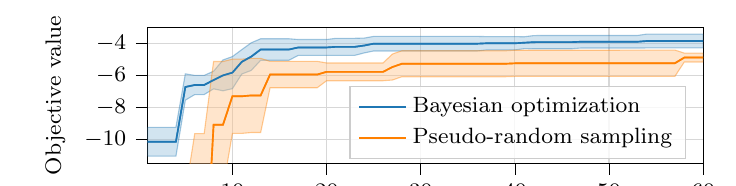
\begin{tikzpicture}[x=1in,y=1in]
  \useasboundingbox (-0.6, 0) rectangle (2.8, -0.65); %
    
  \definecolor{darkgrey176}{RGB}{176,176,176}
  \definecolor{lightgrey204}{RGB}{204,204,204}
  \definecolor{steelblue31119180}{RGB}{31,119,180}

  \begin{axis}[
  anchor=north west,
  width=3.4in,
  height=1.3in,
  legend cell align={left},
  legend style={
    fill opacity=0.8,
    draw opacity=1,
    text opacity=1,
    at={(0.97,0.03)},
    anchor=south east,
    font=\footnotesize,
    draw=lightgrey204
  },
  tick align=outside,
  tick pos=left,
  x grid style={darkgrey176!50},
  xlabel={Episodes},
  xmajorgrids,
  xmin=1, xmax=60,
  xtick style={color=black},
  y grid style={darkgrey176!50},
  ylabel={Objective value},
  ymajorgrids,
  xlabel shift=-1mm,
  ymin=-11.5, ymax=-3.0,
  ytick style={color=black},
  tick label style={font=\footnotesize}, %
  label style={font=\footnotesize}, %
  ]

  \addplot [semithick, steelblue31119180]
  table {%
  1 -10.1574191633144
  2 -10.1574191633144
  3 -10.1574191633144
  4 -10.1574191633144
  5 -6.72289483906331
  6 -6.59684858181106
  7 -6.59684858181106
  8 -6.28596903298211
  9 -5.99373655494911
  10 -5.82167779703389
  11 -5.1428110983115
  12 -4.81673457286373
  13 -4.37088875274734
  14 -4.37088875274734
  15 -4.37088875274734
  16 -4.37088875274734
  17 -4.24148141205882
  18 -4.24148141205882
  19 -4.24148141205882
  20 -4.24148141205882
  21 -4.20245990000189
  22 -4.20245990000189
  23 -4.20245990000189
  24 -4.11959725018268
  25 -4.00556881763445
  26 -4.00556881763445
  27 -4.00556881763445
  28 -4.00556881763445
  29 -4.00556881763445
  30 -4.00556881763445
  31 -4.00556881763445
  32 -4.00556881763445
  33 -4.00556881763445
  34 -4.00556881763445
  35 -4.00556881763445
  36 -4.00556881763445
  37 -3.97949251478588
  38 -3.97949251478588
  39 -3.97949251478588
  40 -3.97949251478588
  41 -3.94404729277079
  42 -3.91049026608397
  43 -3.90720589167441
  44 -3.90720589167441
  45 -3.90720589167441
  46 -3.90720589167441
  47 -3.88429011242476
  48 -3.88429011242476
  49 -3.88429011242476
  50 -3.88429011242476
  51 -3.88429011242476
  52 -3.88429011242476
  53 -3.88429011242476
  54 -3.83778249975218
  55 -3.83778249975218
  56 -3.83778249975218
  57 -3.83778249975218
  58 -3.83778249975218
  59 -3.83778249975218
  60 -3.83778249975218
  };
  \addlegendentry{Bayesian optimization}

  \path [draw=steelblue31119180!100, fill=steelblue31119180!50, opacity=0.4]
  (axis cs:1,-9.25192272947796)
  --(axis cs:1,-11.0629155971508)
  --(axis cs:2,-11.0629155971508)
  --(axis cs:3,-11.0629155971508)
  --(axis cs:4,-11.0629155971508)
  --(axis cs:5,-7.54939492206937)
  --(axis cs:6,-7.19721439515581)
  --(axis cs:7,-7.19721439515581)
  --(axis cs:8,-6.8386905924942)
  --(axis cs:9,-6.96114920237258)
  --(axis cs:10,-6.82854865024866)
  --(axis cs:11,-5.90839733741554)
  --(axis cs:12,-5.68382706642718)
  --(axis cs:13,-5.04568387720924)
  --(axis cs:14,-5.04568387720924)
  --(axis cs:15,-5.04568387720924)
  --(axis cs:16,-5.04568387720924)
  --(axis cs:17,-4.73792464284913)
  --(axis cs:18,-4.73792464284913)
  --(axis cs:19,-4.73792464284913)
  --(axis cs:20,-4.73792464284913)
  --(axis cs:21,-4.73733099029819)
  --(axis cs:22,-4.73733099029819)
  --(axis cs:23,-4.73733099029819)
  --(axis cs:24,-4.58459002120253)
  --(axis cs:25,-4.46280980134367)
  --(axis cs:26,-4.46280980134367)
  --(axis cs:27,-4.46280980134367)
  --(axis cs:28,-4.46280980134367)
  --(axis cs:29,-4.46280980134367)
  --(axis cs:30,-4.46280980134367)
  --(axis cs:31,-4.46280980134367)
  --(axis cs:32,-4.46280980134367)
  --(axis cs:33,-4.46280980134367)
  --(axis cs:34,-4.46280980134367)
  --(axis cs:35,-4.46280980134367)
  --(axis cs:36,-4.46280980134367)
  --(axis cs:37,-4.39831635351107)
  --(axis cs:38,-4.39831635351107)
  --(axis cs:39,-4.39831635351107)
  --(axis cs:40,-4.39831635351107)
  --(axis cs:41,-4.31605252044889)
  --(axis cs:42,-4.32412394230932)
  --(axis cs:43,-4.32527023808848)
  --(axis cs:44,-4.32527023808848)
  --(axis cs:45,-4.32527023808848)
  --(axis cs:46,-4.32527023808848)
  --(axis cs:47,-4.27735676012639)
  --(axis cs:48,-4.27735676012639)
  --(axis cs:49,-4.27735676012639)
  --(axis cs:50,-4.27735676012639)
  --(axis cs:51,-4.27735676012639)
  --(axis cs:52,-4.27735676012639)
  --(axis cs:53,-4.27735676012639)
  --(axis cs:54,-4.27143218019298)
  --(axis cs:55,-4.27143218019298)
  --(axis cs:56,-4.27143218019298)
  --(axis cs:57,-4.27143218019298)
  --(axis cs:58,-4.27143218019298)
  --(axis cs:59,-4.27143218019298)
  --(axis cs:60,-4.27143218019298)
  --(axis cs:60,-3.40413281931137)
  --(axis cs:60,-3.40413281931137)
  --(axis cs:59,-3.40413281931137)
  --(axis cs:58,-3.40413281931137)
  --(axis cs:57,-3.40413281931137)
  --(axis cs:56,-3.40413281931137)
  --(axis cs:55,-3.40413281931137)
  --(axis cs:54,-3.40413281931137)
  --(axis cs:53,-3.49122346472314)
  --(axis cs:52,-3.49122346472314)
  --(axis cs:51,-3.49122346472314)
  --(axis cs:50,-3.49122346472314)
  --(axis cs:49,-3.49122346472314)
  --(axis cs:48,-3.49122346472314)
  --(axis cs:47,-3.49122346472314)
  --(axis cs:46,-3.48914154526035)
  --(axis cs:45,-3.48914154526035)
  --(axis cs:44,-3.48914154526035)
  --(axis cs:43,-3.48914154526035)
  --(axis cs:42,-3.49685658985863)
  --(axis cs:41,-3.57204206509268)
  --(axis cs:40,-3.56066867606069)
  --(axis cs:39,-3.56066867606069)
  --(axis cs:38,-3.56066867606069)
  --(axis cs:37,-3.56066867606069)
  --(axis cs:36,-3.54832783392523)
  --(axis cs:35,-3.54832783392523)
  --(axis cs:34,-3.54832783392523)
  --(axis cs:33,-3.54832783392523)
  --(axis cs:32,-3.54832783392523)
  --(axis cs:31,-3.54832783392523)
  --(axis cs:30,-3.54832783392523)
  --(axis cs:29,-3.54832783392523)
  --(axis cs:28,-3.54832783392523)
  --(axis cs:27,-3.54832783392523)
  --(axis cs:26,-3.54832783392523)
  --(axis cs:25,-3.54832783392523)
  --(axis cs:24,-3.65460447916283)
  --(axis cs:23,-3.6675888097056)
  --(axis cs:22,-3.6675888097056)
  --(axis cs:21,-3.6675888097056)
  --(axis cs:20,-3.74503818126851)
  --(axis cs:19,-3.74503818126851)
  --(axis cs:18,-3.74503818126851)
  --(axis cs:17,-3.74503818126851)
  --(axis cs:16,-3.69609362828544)
  --(axis cs:15,-3.69609362828544)
  --(axis cs:14,-3.69609362828544)
  --(axis cs:13,-3.69609362828544)
  --(axis cs:12,-3.94964207930029)
  --(axis cs:11,-4.37722485920747)
  --(axis cs:10,-4.81480694381912)
  --(axis cs:9,-5.02632390752564)
  --(axis cs:8,-5.73324747347001)
  --(axis cs:7,-5.99648276846631)
  --(axis cs:6,-5.99648276846631)
  --(axis cs:5,-5.89639475605725)
  --(axis cs:4,-9.25192272947796)
  --(axis cs:3,-9.25192272947796)
  --(axis cs:2,-9.25192272947796)
  --(axis cs:1,-9.25192272947796)
  --cycle;

  \addplot [semithick, orange]
  table {%
  1 -24.8117548316848
  2 -24.8117548316848
  3 -24.8117548316848
  4 -24.8117548316848
  5 -23.9097738609303
  6 -20.0768245547915
  7 -20.0768245547915
  8 -9.09489985281767
  9 -9.09489985281767
  10 -7.30449400207115
  11 -7.30449400207115
  12 -7.25275367414012
  13 -7.25275367414012
  14 -5.94324016597094
  15 -5.94324016597094
  16 -5.94324016597094
  17 -5.94324016597094
  18 -5.94324016597094
  19 -5.94324016597094
  20 -5.77141780882547
  21 -5.77141780882547
  22 -5.77141780882547
  23 -5.77141780882547
  24 -5.77141780882547
  25 -5.77141780882547
  26 -5.77141780882547
  27 -5.46955325648097
  28 -5.26388748129056
  29 -5.26388748129056
  30 -5.26388748129056
  31 -5.26388748129056
  32 -5.26388748129056
  33 -5.26388748129056
  34 -5.26388748129056
  35 -5.26388748129056
  36 -5.26388748129056
  37 -5.26388748129056
  38 -5.26388748129056
  39 -5.26388748129056
  40 -5.23696661156889
  41 -5.23696661156889
  42 -5.23696661156889
  43 -5.23696661156889
  44 -5.23696661156889
  45 -5.23696661156889
  46 -5.23696661156889
  47 -5.23696661156889
  48 -5.23696661156889
  49 -5.23696661156889
  50 -5.23696661156889
  51 -5.23696661156889
  52 -5.22987952313497
  53 -5.22987952313497
  54 -5.22987952313497
  55 -5.22987952313497
  56 -5.22987952313497
  57 -5.22987952313497
  58 -4.8758610705042
  59 -4.8758610705042
  60 -4.8758610705042
  };
  \addlegendentry{Pseudo-random sampling}

  \path [draw=orange!100, fill=orange!50, opacity=0.4]
  (axis cs:1,-15.8254505980391)
  --(axis cs:1,-33.7980590653305)
  --(axis cs:2,-33.7980590653305)
  --(axis cs:3,-33.7980590653305)
  --(axis cs:4,-33.7980590653305)
  --(axis cs:5,-34.4583549633831)
  --(axis cs:6,-30.500835698174)
  --(axis cs:7,-30.500835698174)
  --(axis cs:8,-13.0650976691005)
  --(axis cs:9,-13.0650976691005)
  --(axis cs:10,-9.63305186269427)
  --(axis cs:11,-9.63305186269427)
  --(axis cs:12,-9.57854407058712)
  --(axis cs:13,-9.57854407058712)
  --(axis cs:14,-6.7726501658824)
  --(axis cs:15,-6.7726501658824)
  --(axis cs:16,-6.7726501658824)
  --(axis cs:17,-6.7726501658824)
  --(axis cs:18,-6.7726501658824)
  --(axis cs:19,-6.7726501658824)
  --(axis cs:20,-6.32853325564196)
  --(axis cs:21,-6.32853325564196)
  --(axis cs:22,-6.32853325564196)
  --(axis cs:23,-6.32853325564196)
  --(axis cs:24,-6.32853325564196)
  --(axis cs:25,-6.32853325564196)
  --(axis cs:26,-6.32853325564196)
  --(axis cs:27,-6.28418882407104)
  --(axis cs:28,-6.07760333508252)
  --(axis cs:29,-6.07760333508252)
  --(axis cs:30,-6.07760333508252)
  --(axis cs:31,-6.07760333508252)
  --(axis cs:32,-6.07760333508252)
  --(axis cs:33,-6.07760333508252)
  --(axis cs:34,-6.07760333508252)
  --(axis cs:35,-6.07760333508252)
  --(axis cs:36,-6.07760333508252)
  --(axis cs:37,-6.07760333508252)
  --(axis cs:38,-6.07760333508252)
  --(axis cs:39,-6.07760333508252)
  --(axis cs:40,-6.05896797065684)
  --(axis cs:41,-6.05896797065684)
  --(axis cs:42,-6.05896797065684)
  --(axis cs:43,-6.05896797065684)
  --(axis cs:44,-6.05896797065684)
  --(axis cs:45,-6.05896797065684)
  --(axis cs:46,-6.05896797065684)
  --(axis cs:47,-6.05896797065684)
  --(axis cs:48,-6.05896797065684)
  --(axis cs:49,-6.05896797065684)
  --(axis cs:50,-6.05896797065684)
  --(axis cs:51,-6.05896797065684)
  --(axis cs:52,-6.05436508485352)
  --(axis cs:53,-6.05436508485352)
  --(axis cs:54,-6.05436508485352)
  --(axis cs:55,-6.05436508485352)
  --(axis cs:56,-6.05436508485352)
  --(axis cs:57,-6.05436508485352)
  --(axis cs:58,-5.15323923666181)
  --(axis cs:59,-5.15323923666181)
  --(axis cs:60,-5.15323923666181)
  --(axis cs:60,-4.59848290434659)
  --(axis cs:60,-4.59848290434659)
  --(axis cs:59,-4.59848290434659)
  --(axis cs:58,-4.59848290434659)
  --(axis cs:57,-4.40539396141641)
  --(axis cs:56,-4.40539396141641)
  --(axis cs:55,-4.40539396141641)
  --(axis cs:54,-4.40539396141641)
  --(axis cs:53,-4.40539396141641)
  --(axis cs:52,-4.40539396141641)
  --(axis cs:51,-4.41496525248093)
  --(axis cs:50,-4.41496525248093)
  --(axis cs:49,-4.41496525248093)
  --(axis cs:48,-4.41496525248093)
  --(axis cs:47,-4.41496525248093)
  --(axis cs:46,-4.41496525248093)
  --(axis cs:45,-4.41496525248093)
  --(axis cs:44,-4.41496525248093)
  --(axis cs:43,-4.41496525248093)
  --(axis cs:42,-4.41496525248093)
  --(axis cs:41,-4.41496525248093)
  --(axis cs:40,-4.41496525248093)
  --(axis cs:39,-4.45017162749861)
  --(axis cs:38,-4.45017162749861)
  --(axis cs:37,-4.45017162749861)
  --(axis cs:36,-4.45017162749861)
  --(axis cs:35,-4.45017162749861)
  --(axis cs:34,-4.45017162749861)
  --(axis cs:33,-4.45017162749861)
  --(axis cs:32,-4.45017162749861)
  --(axis cs:31,-4.45017162749861)
  --(axis cs:30,-4.45017162749861)
  --(axis cs:29,-4.45017162749861)
  --(axis cs:28,-4.45017162749861)
  --(axis cs:27,-4.65491768889089)
  --(axis cs:26,-5.21430236200899)
  --(axis cs:25,-5.21430236200899)
  --(axis cs:24,-5.21430236200899)
  --(axis cs:23,-5.21430236200899)
  --(axis cs:22,-5.21430236200899)
  --(axis cs:21,-5.21430236200899)
  --(axis cs:20,-5.21430236200899)
  --(axis cs:19,-5.11383016605948)
  --(axis cs:18,-5.11383016605948)
  --(axis cs:17,-5.11383016605948)
  --(axis cs:16,-5.11383016605948)
  --(axis cs:15,-5.11383016605948)
  --(axis cs:14,-5.11383016605948)
  --(axis cs:13,-4.92696327769312)
  --(axis cs:12,-4.92696327769312)
  --(axis cs:11,-4.97593614144803)
  --(axis cs:10,-4.97593614144803)
  --(axis cs:9,-5.12470203653484)
  --(axis cs:8,-5.12470203653484)
  --(axis cs:7,-9.65281341140902)
  --(axis cs:6,-9.65281341140902)
  --(axis cs:5,-13.3611927584774)
  --(axis cs:4,-15.8254505980391)
  --(axis cs:3,-15.8254505980391)
  --(axis cs:2,-15.8254505980391)
  --(axis cs:1,-15.8254505980391)
  --cycle;


  \addplot [semithick, steelblue31119180]
  table {%
  1 -10.1574191633144
  2 -10.1574191633144
  3 -10.1574191633144
  4 -10.1574191633144
  5 -6.72289483906331
  6 -6.59684858181106
  7 -6.59684858181106
  8 -6.28596903298211
  9 -5.99373655494911
  10 -5.82167779703389
  11 -5.1428110983115
  12 -4.81673457286373
  13 -4.37088875274734
  14 -4.37088875274734
  15 -4.37088875274734
  16 -4.37088875274734
  17 -4.24148141205882
  18 -4.24148141205882
  19 -4.24148141205882
  20 -4.24148141205882
  21 -4.20245990000189
  22 -4.20245990000189
  23 -4.20245990000189
  24 -4.11959725018268
  25 -4.00556881763445
  26 -4.00556881763445
  27 -4.00556881763445
  28 -4.00556881763445
  29 -4.00556881763445
  30 -4.00556881763445
  31 -4.00556881763445
  32 -4.00556881763445
  33 -4.00556881763445
  34 -4.00556881763445
  35 -4.00556881763445
  36 -4.00556881763445
  37 -3.97949251478588
  38 -3.97949251478588
  39 -3.97949251478588
  40 -3.97949251478588
  41 -3.94404729277079
  42 -3.91049026608397
  43 -3.90720589167441
  44 -3.90720589167441
  45 -3.90720589167441
  46 -3.90720589167441
  47 -3.88429011242476
  48 -3.88429011242476
  49 -3.88429011242476
  50 -3.88429011242476
  51 -3.88429011242476
  52 -3.88429011242476
  53 -3.88429011242476
  54 -3.83778249975218
  55 -3.83778249975218
  56 -3.83778249975218
  57 -3.83778249975218
  58 -3.83778249975218
  59 -3.83778249975218
  60 -3.83778249975218
  };
  


  \addplot [semithick, orange]
  table {%
  1 -24.8117548316848
  2 -24.8117548316848
  3 -24.8117548316848
  4 -24.8117548316848
  5 -23.9097738609303
  6 -20.0768245547915
  7 -20.0768245547915
  8 -9.09489985281767
  9 -9.09489985281767
  10 -7.30449400207115
  11 -7.30449400207115
  12 -7.25275367414012
  13 -7.25275367414012
  14 -5.94324016597094
  15 -5.94324016597094
  16 -5.94324016597094
  17 -5.94324016597094
  18 -5.94324016597094
  19 -5.94324016597094
  20 -5.77141780882547
  21 -5.77141780882547
  22 -5.77141780882547
  23 -5.77141780882547
  24 -5.77141780882547
  25 -5.77141780882547
  26 -5.77141780882547
  27 -5.46955325648097
  28 -5.26388748129056
  29 -5.26388748129056
  30 -5.26388748129056
  31 -5.26388748129056
  32 -5.26388748129056
  33 -5.26388748129056
  34 -5.26388748129056
  35 -5.26388748129056
  36 -5.26388748129056
  37 -5.26388748129056
  38 -5.26388748129056
  39 -5.26388748129056
  40 -5.23696661156889
  41 -5.23696661156889
  42 -5.23696661156889
  43 -5.23696661156889
  44 -5.23696661156889
  45 -5.23696661156889
  46 -5.23696661156889
  47 -5.23696661156889
  48 -5.23696661156889
  49 -5.23696661156889
  50 -5.23696661156889
  51 -5.23696661156889
  52 -5.22987952313497
  53 -5.22987952313497
  54 -5.22987952313497
  55 -5.22987952313497
  56 -5.22987952313497
  57 -5.22987952313497
  58 -4.8758610705042
  59 -4.8758610705042
  60 -4.8758610705042
  };
  
  
  \addplot [very thick, black, dash pattern=on 11.1pt off 4.8pt]
  table {%
  0 0
  59 0
  };
  \end{axis}

  \end{tikzpicture}

\clearpage
\section{Text capabilities }\label{sec:text_ability}
We assess the text-related capabilities of \ourM{} (8x7B) in this section. We first present several examples to provide readers with an intuitive understanding (Section \ref{sec:case_study}), and then benchmark results from AlpacaEval (Section \ref{sec:alpahaeval}).

\subsection{Case study}\label{sec:case_study}
%\TODO{@Yuan-Jyue}, pls input several text cases here.
Here we demonstrate our model's language capabilities in scientific discovery research. Specifically, we assessed the model's understanding of CRISPR gene editing, cancer immunotherapy, and drug discovery. A few selected cases are presented in this section for brevity. Additional cases can be found in Fig. \ref{SI_fig:case_study:CRISPR}, \ref{SI_fig:case_study:cancer_immunotherapy} and \ref{SI_fig:case_study:drug_discovery}.


\subsubsection{CRISPR gene editing}
 CRISPR gene editing has rapidly emerged as a powerful tool in biotechnology. Our model demonstrates a good understanding of CRISPR and is able to effectively analyze the advantages and disadvantages of commonly used CRISPR tools. 

  
\begin{mdframed}[backgroundcolor=white, linecolor=black, linewidth=1pt]
    \noindent
    \textbf{Instruction:} Could you provide me the advantages and disadvantages of Cas9? \\
    \textbf{Response:} \\
    Advantages: 1. Highly efficient and specific gene editing with a low risk of off-target effects. 2. Can target a wide range of sequences.  3. Cam be used to make specific alterations to genes in virtually any organism.  Disadvantages: 1. Potential for off-target effects when using Cas9. 2. The delivery of Cas9 can be inefficient. 3. Lack of control over the repair mechanism. 4. May cause chromosomal abnormalities. \\

    \noindent
    \textbf{Instruction:} Could you provide me the advantages and disadvantages of Cas12a, another widely used CRISPR protein? \\
    \textbf{Response:} \\
    Advantages: \\
    1. High specificty: Cas12a has higher specificity compared to Cas 9, which reduces off-target effects. 
    2. Simpler PAM requirements: Cas 12a requires a simpler PAM sequence than Cas9, making it easier to target specific genomic loci. 
    3. Multiplexing: Cas12a can be used for multiplexing genome editing, meaning multiple genomic loci can be edited in a single reaction. 
    Disadvantages: \\
    4. Lower efficiency: Cas12a is less efficient in terms of indel formation than Cas9. 
    5. Larger size: Cas12a is a larger protein than Cas9, which can make it harder to deliver the Cas12a system into cells. \\
    ... 
\end{mdframed}  
\captionof{figure}{Cases about CRISPR gene editing.} \label{fig:case_study:CRISPR}

\subsubsection{Cancer immunotherapy}
Our model is knowledgeable about existing checkpoint inhibitors used in cancer therapy and provides accurate explanations of their mechanisms of action. Specifically, in our experiment, it generates a valid peptide sequence for inhibiting the overexpressed PD-L1 protein (see Figure \ref{SI_fig:case_study:cancer_immunotherapy}), although the length of the peptide is incorrect. It demonstrates a solid understanding of the inhibition cascade between drugs and proteins.

\begin{mdframed}[backgroundcolor=white, linecolor=black, linewidth=1pt]  
    \noindent
    \textbf{Instruction:} Tell me existing checkpoint inhibitors for PD-L1. \\
    \textbf{Response:} The checkpoint inhibitors for PD-L1 that are currently approved by the FDA include atezolizumab, avelumab, duravalumab, and perbrolizumab.\\
    
    \noindent
    \textbf{Instruction:} PD-L1 is a protein that inhibits PD-1, a recptor found on T cells. This new drug X, is designed to inhibit PD-L1. If we introduce drug X, will T cell function be restored? Explain it step by step. \\
    \textbf{Response:}
    PD-1 is inhibited by interaction with PD-L1. If drug X inhibits PD-L1, PD-1 will no longer be inhibited. Therefore, T cell function will beestored. Therefore, the answer is yes.

\end{mdframed}  
\captionof{figure}{Cases about cancer immunotherapy.} \label{fig:case_study:cancer_immunotherapy}

\subsubsection{Drug discovery}
Drug discovery is an evolving process that incorporates empirical rules, computational design, and experimental validation. The model demonstrates an understanding of the fundamental principles of drug discovery. Specifically, when being asked questions about Lipinski’s Rule of Five and strategies (see Figure \ref{SI_fig:case_study:drug_discovery}) to improve a drug’s ADME properties, the model provides mostly accurate answers.

\begin{mdframed}[backgroundcolor=white, linecolor=black, linewidth=1pt]  
    \textbf{Instruction:} What approaches can drug experts use to enhance a drug's ADME properties? \\
    \textbf{Response:} Structure-based drug design: Computational techniques can be used to modify existing drugs or design new ones with desired ADME properties. 2. Lipophilicity: Lipophilicity can affect the ADME profile of a drug. 3. Hepatic and extracellular clearance: Understanding the hepatic and extracellular clearance of a drug is important for assessing its ADME profile. 4. Microsomal stability: Microsomal stability is a measure of how quickly a drug is broken down by liver enzymes. 5. Oral absorption: Oral absorption is determined by the solubility and permeability of a drug. 6. Permeability: The ability of a drug to cross cell membranes affects its bioavailability. 
    ... %7. Plasma protein binding: Plasma protein binding affects the concentration of free drug available to interact with its target. 8. Efflux transporters: Efflux transporters can affect the absorption, distribution, and excretion of a drug. 

\end{mdframed}  
\captionof{figure}{Case about drug discovery.} \label{fig:case_study:drug
_discovery}

\subsection{Comparison on AlpacaEval evaluation}\label{sec:alpahaeval}
To assess the linguistic capabilities of \ourM{}, we compared \ourM{} (8x7B) with the original Mixtral  (8x7B) using the AlpacaEval \cite{dubois2024length} dataset and method. AlpacaEval is a benchmark for LLM designed to gauge a model's proficiency in executing general user instructions. \ourM{}'s responses are compared against reference responses generated by original Mixtral using GPT-4 as the annotator. We focused on two metrics from AlpacaEval: the general win rate and the LC win rate (length-controlled win rate), which controls the bias introduced by the length of the responses. Our NatureLM model achieved a LC win rate of 31.8\% and a win rate of 25.2\% when benchmarked against Mixtral, showcasing that while the model possesses a foundational level of language comprehension, it exhibits constraints in its linguistic capacity.   A potential contributing factor to this limited performance is the overrepresentation of scientific data within the training dataset, which may skew the model's proficiency towards technical language and away from a more generalized understanding required for diverse user instructions. Fig. \ref{fig:case_study:alpacaeval} presents two illustrative examples from the AlpacaEval comparison. We will improve the text capabilities of \ourM{} in our future work. 

\clearpage
\section{Discussion of Assumptions}\label{sec:discussion}
In this paper, we have made several assumptions for the sake of clarity and simplicity. In this section, we discuss the rationale behind these assumptions, the extent to which these assumptions hold in practice, and the consequences for our protocol when these assumptions hold.

\subsection{Assumptions on the Demand}

There are two simplifying assumptions we make about the demand. First, we assume the demand at any time is relatively small compared to the channel capacities. Second, we take the demand to be constant over time. We elaborate upon both these points below.

\paragraph{Small demands} The assumption that demands are small relative to channel capacities is made precise in \eqref{eq:large_capacity_assumption}. This assumption simplifies two major aspects of our protocol. First, it largely removes congestion from consideration. In \eqref{eq:primal_problem}, there is no constraint ensuring that total flow in both directions stays below capacity--this is always met. Consequently, there is no Lagrange multiplier for congestion and no congestion pricing; only imbalance penalties apply. In contrast, protocols in \cite{sivaraman2020high, varma2021throughput, wang2024fence} include congestion fees due to explicit congestion constraints. Second, the bound \eqref{eq:large_capacity_assumption} ensures that as long as channels remain balanced, the network can always meet demand, no matter how the demand is routed. Since channels can rebalance when necessary, they never drop transactions. This allows prices and flows to adjust as per the equations in \eqref{eq:algorithm}, which makes it easier to prove the protocol's convergence guarantees. This also preserves the key property that a channel's price remains proportional to net money flow through it.

In practice, payment channel networks are used most often for micro-payments, for which on-chain transactions are prohibitively expensive; large transactions typically take place directly on the blockchain. For example, according to \cite{river2023lightning}, the average channel capacity is roughly $0.1$ BTC ($5,000$ BTC distributed over $50,000$ channels), while the average transaction amount is less than $0.0004$ BTC ($44.7k$ satoshis). Thus, the small demand assumption is not too unrealistic. Additionally, the occasional large transaction can be treated as a sequence of smaller transactions by breaking it into packets and executing each packet serially (as done by \cite{sivaraman2020high}).
Lastly, a good path discovery process that favors large capacity channels over small capacity ones can help ensure that the bound in \eqref{eq:large_capacity_assumption} holds.

\paragraph{Constant demands} 
In this work, we assume that any transacting pair of nodes have a steady transaction demand between them (see Section \ref{sec:transaction_requests}). Making this assumption is necessary to obtain the kind of guarantees that we have presented in this paper. Unless the demand is steady, it is unreasonable to expect that the flows converge to a steady value. Weaker assumptions on the demand lead to weaker guarantees. For example, with the more general setting of stochastic, but i.i.d. demand between any two nodes, \cite{varma2021throughput} shows that the channel queue lengths are bounded in expectation. If the demand can be arbitrary, then it is very hard to get any meaningful performance guarantees; \cite{wang2024fence} shows that even for a single bidirectional channel, the competitive ratio is infinite. Indeed, because a PCN is a decentralized system and decisions must be made based on local information alone, it is difficult for the network to find the optimal detailed balance flow at every time step with a time-varying demand.  With a steady demand, the network can discover the optimal flows in a reasonably short time, as our work shows.

We view the constant demand assumption as an approximation for a more general demand process that could be piece-wise constant, stochastic, or both (see simulations in Figure \ref{fig:five_nodes_variable_demand}).
We believe it should be possible to merge ideas from our work and \cite{varma2021throughput} to provide guarantees in a setting with random demands with arbitrary means. We leave this for future work. In addition, our work suggests that a reasonable method of handling stochastic demands is to queue the transaction requests \textit{at the source node} itself. This queuing action should be viewed in conjunction with flow-control. Indeed, a temporarily high unidirectional demand would raise prices for the sender, incentivizing the sender to stop sending the transactions. If the sender queues the transactions, they can send them later when prices drop. This form of queuing does not require any overhaul of the basic PCN infrastructure and is therefore simpler to implement than per-channel queues as suggested by \cite{sivaraman2020high} and \cite{varma2021throughput}.

\subsection{The Incentive of Channels}
The actions of the channels as prescribed by the DEBT control protocol can be summarized as follows. Channels adjust their prices in proportion to the net flow through them. They rebalance themselves whenever necessary and execute any transaction request that has been made of them. We discuss both these aspects below.

\paragraph{On Prices}
In this work, the exclusive role of channel prices is to ensure that the flows through each channel remains balanced. In practice, it would be important to include other components in a channel's price/fee as well: a congestion price  and an incentive price. The congestion price, as suggested by \cite{varma2021throughput}, would depend on the total flow of transactions through the channel, and would incentivize nodes to balance the load over different paths. The incentive price, which is commonly used in practice \cite{river2023lightning}, is necessary to provide channels with an incentive to serve as an intermediary for different channels. In practice, we expect both these components to be smaller than the imbalance price. Consequently, we expect the behavior of our protocol to be similar to our theoretical results even with these additional prices.

A key aspect of our protocol is that channel fees are allowed to be negative. Although the original Lightning network whitepaper \cite{poon2016bitcoin} suggests that negative channel prices may be a good solution to promote rebalancing, the idea of negative prices in not very popular in the literature. To our knowledge, the only prior work with this feature is \cite{varma2021throughput}. Indeed, in papers such as \cite{van2021merchant} and \cite{wang2024fence}, the price function is explicitly modified such that the channel price is never negative. The results of our paper show the benefits of negative prices. For one, in steady state, equal flows in both directions ensure that a channel doesn't loose any money (the other price components mentioned above ensure that the channel will only gain money). More importantly, negative prices are important to ensure that the protocol selectively stifles acyclic flows while allowing circulations to flow. Indeed, in the example of Section \ref{sec:flow_control_example}, the flows between nodes $A$ and $C$ are left on only because the large positive price over one channel is canceled by the corresponding negative price over the other channel, leading to a net zero price.

Lastly, observe that in the DEBT control protocol, the price charged by a channel does not depend on its capacity. This is a natural consequence of the price being the Lagrange multiplier for the net-zero flow constraint, which also does not depend on the channel capacity. In contrast, in many other works, the imbalance price is normalized by the channel capacity \cite{ren2018optimal, lin2020funds, wang2024fence}; this is shown to work well in practice. The rationale for such a price structure is explained well in \cite{wang2024fence}, where this fee is derived with the aim of always maintaining some balance (liquidity) at each end of every channel. This is a reasonable aim if a channel is to never rebalance itself; the experiments of the aforementioned papers are conducted in such a regime. In this work, however, we allow the channels to rebalance themselves a few times in order to settle on a detailed balance flow. This is because our focus is on the long-term steady state performance of the protocol. This difference in perspective also shows up in how the price depends on the channel imbalance. \cite{lin2020funds} and \cite{wang2024fence} advocate for strictly convex prices whereas this work and \cite{varma2021throughput} propose linear prices.

\paragraph{On Rebalancing} 
Recall that the DEBT control protocol ensures that the flows in the network converge to a detailed balance flow, which can be sustained perpetually without any rebalancing. However, during the transient phase (before convergence), channels may have to perform on-chain rebalancing a few times. Since rebalancing is an expensive operation, it is worthwhile discussing methods by which channels can reduce the extent of rebalancing. One option for the channels to reduce the extent of rebalancing is to increase their capacity; however, this comes at the cost of locking in more capital. Each channel can decide for itself the optimum amount of capital to lock in. Another option, which we discuss in Section \ref{sec:five_node}, is for channels to increase the rate $\gamma$ at which they adjust prices. 

Ultimately, whether or not it is beneficial for a channel to rebalance depends on the time-horizon under consideration. Our protocol is based on the assumption that the demand remains steady for a long period of time. If this is indeed the case, it would be worthwhile for a channel to rebalance itself as it can make up this cost through the incentive fees gained from the flow of transactions through it in steady state. If a channel chooses not to rebalance itself, however, there is a risk of being trapped in a deadlock, which is suboptimal for not only the nodes but also the channel.

\section{Conclusion}
This work presents DEBT control: a protocol for payment channel networks that uses source routing and flow control based on channel prices. The protocol is derived by posing a network utility maximization problem and analyzing its dual minimization. It is shown that under steady demands, the protocol guides the network to an optimal, sustainable point. Simulations show its robustness to demand variations. The work demonstrates that simple protocols with strong theoretical guarantees are possible for PCNs and we hope it inspires further theoretical research in this direction.


\clearpage
\bibliography{sn-bibliography}

\clearpage
\appendix
\setcounter{figure}{0}  % reset counter  
\renewcommand{\thefigure}{S\arabic{figure}}
\setcounter{table}{0}  % reset counter  
\renewcommand{\thetable}{S\arabic{table}} % changes table 1 to table S1  % changes figure 1 to figure S1 
\begin{appendices}

\setcounter{section}{0}
\renewcommand{\thesection}{SI}
%\renewcommand{\thesubsection}{SI.\arabic{subsection}}
\renewcommand{\thesubsection}{\Alph{subsection}}

\renewcommand{\thetable}{S\arabic{table}}
\setcounter{table}{0}  % Reset table counter to start from 1
\renewcommand{\thefigure}{S\arabic{figure}}
\setcounter{figure}{0}



\section{Supplemental Material}

\subsection{Data Collection}

\subsubsection{Obtaining Observational Studies}

This study adopts the definition of {\em an observational study} provided by
the NIH National Library of Medicine\footnote{https://www.ncbi.nlm.nih.gov/mesh/68064888},
which states:
``[...] a work that reports on the results of a clinical study
in which participants may receive diagnostic, therapeutic, or other types of interventions,
but the investigator does not assign participants to specific interventions (as in an interventional study).''

We initially retrieved 160,256 papers from the PubMed database using the query
{\em Observational Study[Publication Type]} via the Entrez system. The majority
of these papers were published in 2014 or later, following the
introduction of the MeSH term {\em Observational Study}. We then excluded
publications that were also labeled as {\em Randomized Controlled Trial} or {\em
Clinical Trial}, leaving us with 155,933 exclusive observational studies. Next,
we removed papers that lacked either a structured abstract with a conclusion
subsection or an English full text, resulting in 104,508 observational studies
with a {\em Conclusion(s)} subsection and English full text. Finally, we
excluded articles whose conclusions did not contain any causal or correlational
claims—typically those focused solely on descriptive findings, recommendations,
study implications, or future work. This filtering process resulted in a final
dataset of 81,132 observational studies for analysis (see
Fig.~\ref{fig__flowchart_data_collection}).


\begin{figure}[!ht]
\centering
	
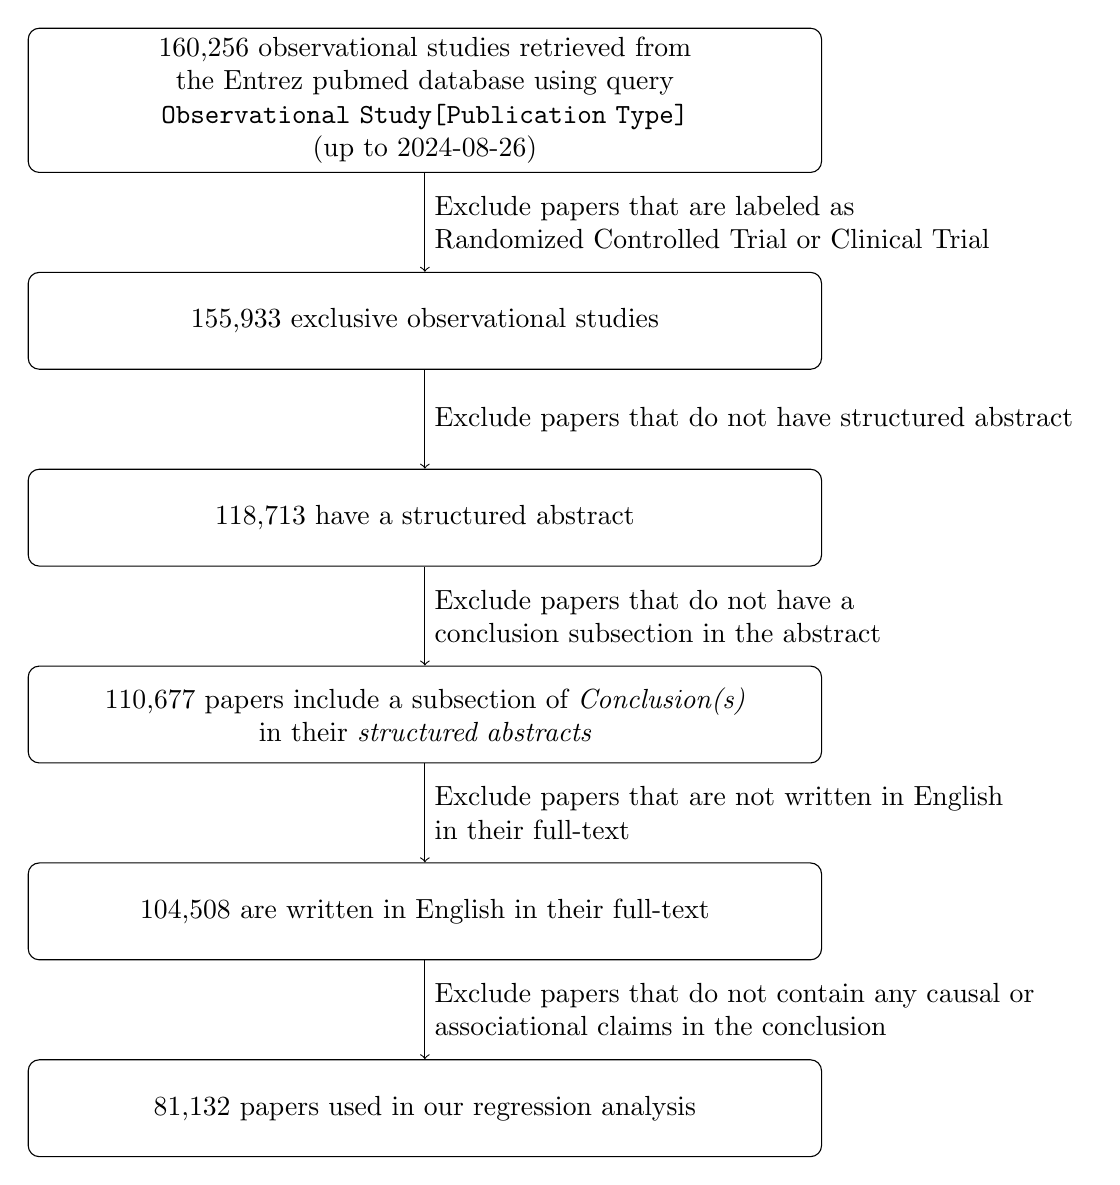
\begin{tikzpicture}
    \tikzstyle{block} = [rectangle, rounded corners, draw, text width=28em, text centered, minimum height=3.5em]

    % Place nodes
    \node [block] (block1) {160,256 observational studies retrieved from the Entrez pubmed database
    using query {\tt Observational Study[Publication Type]} \\
    (up to 2024-08-26)};
    
    \node [block, below of=block1, yshift=-1.8cm] (block2) {
        155,933 exclusive observational studies
    };
    
    \node [block, below of=block2, yshift=-1.5cm] (block2_3) {
        118,713 have a structured abstract \\ 
    };
    \node [block, below of=block2_3, yshift=-1.5cm] (block3) {
        110,677 papers include a subsection of {\em Conclusion(s)} \\ in their {\em structured abstracts}
    };
    \node [block, below of=block3, yshift=-1.5cm] (block4) {
        104,508 are written in English in their full-text
    };
    \node [block, below of=block4, yshift=-1.5cm] (block5) {
        81,132 papers used in our regression analysis
    };

    \draw[->] (block1) -- (block2) node[anchor=west, midway, align=left] {
        Exclude papers that are labeled as \\ Randomized Controlled Trial or Clinical Trial
    };
    
    \draw[->] (block2) -- (block2_3) node[anchor=west, midway, align=left] {
        Exclude papers that do not have structured abstract 
    };

    \draw[->] (block2_3) -- (block3) node[anchor=west, midway, align=left] {
        Exclude papers that do not have a \\ conclusion subsection in the abstract
    };

    \draw[->] (block3) -- (block4) node[anchor=west, midway, align=left] {
        Exclude papers that are not written in English \\ in their full-text
    };

    \draw[->] (block4) -- (block5) node[anchor=west, midway, align=left] {
        Exclude papers that do not contain any causal or \\
        associational claims in the conclusion 
    };

\end{tikzpicture}

	\caption{The process of collecting the observational studies for our analysis.}
	\label{fig__flowchart_data_collection}
\end{figure}


\subsubsection{Journal Rank}

We downloaded publicly accessible SciMago Journal Rank (SJR) data for 2023 and
prior years\footnote{https://www.scimagojr.com/journalrank.php}. For journals in
our dataset that could not be matched to the 2023 data via their ISSN, we
attempted to retrieve their information from previous years. If a journal
remained unmatched (which occurred for only 0.35\% of the papers), we assigned
it an SJR score of 0.47, corresponding to the bottom quartile in our list of
2,629 journals, based on the assumption that journals not listed in the SJR
database are likely to have a low rank.

\subsubsection{Author Writing Experience and Name Disambiguation}

An author’s writing experience is measured by the number of observational
studies they are associated with in our dataset.
To disambiguate author names, we used the
Semantic Scholar API\footnote{https://api.semanticscholar.org/} to obtain a
unique ID for each author per article. Author IDs were successfully retrieved
for 99.8\% of the authors; for the remainder, a unique random ID was generated
and assigned.



%%%%%%%%%%%%%%%%%%%%%%%
% 222
\subsection{Data Preprocessing}

\subsubsection{Causal and Correlational Claim Identification} \label{si_causal_or_correlational}

Building on our previous work  \citep{yu2019EMNLPCausalLanguage} 
and the taxonomy introduced in \citep{sumner2014association,li2017nlp}, we
curated a corpus of 3,061 sentences exemplifying causal language. Using this
dataset, we developed a BioBERT-based
model\footnote{https://github.com/junwang4/causal-language-use-in-science} to
classify a sentence in the conclusion subsection of an abstract into four levels
of claim strength: Causal, Conditional Causal, Correlational, or None. 
A “causal” claim uses terms indicating direct causation (e.g., {\em increase,
make, lead to, effective in, contribute to}) or uses the modal verb {\em can}
followed by a causal verb. A “conditional” claim uses qualifiers (e.g., {\em
may, might, appear to, probably}) to tone down the level of certainty, whereas a
“correlational” claim employs language suggesting an association (e.g., {\em
associated with, predictor, linked with}).

For this study, we merged the “conditional causal” and “correlational”
categories into a single “correlational” category, based on previous research
indicating that general readers often have difficulty distinguishing between these
two \citep{adams2017readers, bratton2020causal}. With this modification, we
fine-tuned the BioBERT-based model using the same training corpus and evaluation
procedure described in \citep{yu2019EMNLPCausalLanguage}, achieving a macro-F1
score of 0.89. Moreover, two empirical comparisons with the ChatGPT family of
models demonstrated that our specifically trained model still have advantages over ChatGPT for
this task \citep{kim2023can, chen2024evaluating}.

In our analysis, if a structured abstract’s conclusion subsection contains two
or more sentences (which occurs in 70.2\% of our dataset) and at least one
sentence is classified as causal, the entire conclusion is considered to include
a causal claim. Based on this criterion, 31.0\% of the 81,132 conclusions
contain a causal claim.

%---------------------
% 22b
\subsubsection{Country Label} \label{si_country}

Author affiliations in the PubMed metadata provide a basis for inferring country
information. However, this can be challenging when the country is not explicitly
mentioned (e.g., “Beth Israel Deaconess Medical Center”). To address this, we
developed an algorithm to infer the country associated with an author’s
affiliation, trained on a dataset of 2.7 million organizations with known
country information from the ORCID
database\footnote{https://support.orcid.org/hc/en-us/articles/360006897394-How-do-I-get-the-public-data-file}.

We evaluated the algorithm using 1,000 randomly sampled affiliations from the
PubMed metadata. These affiliations fell into two categories: (1) those with
insufficient information to infer the country (e.g., “Division of Infectious
Diseases”) and (2) those with sufficient information. For the few cases (7
affiliations) in Category 1, the algorithm output low confidence (less than
0.8), whereas for Category 2, all inferences were accurate. For additional
details, please visit our GitHub
page\footnote{https://github.com/junwang4/affiliation-to-country-inference}.

For each paper, if all author affiliations are classified under the same country
and the average confidence score exceeds 0.8, the paper is labeled with that
country; otherwise, it is labeled as “others.”
Fig.~\ref{fig__country_distribution} shows the distribution of countries that
have published at least 300 observational studies.

\begin{figure}[!ht]
    \includegraphics[width=.9\textwidth]{./figure/country_distri_R.pdf}
        \caption{
        Number of observational studies by authors from 27 exclusive countries that
        have published at least 300 papers in our dataset, along with the “others” category.
        The “others” category includes 23,153 observational studies: 
        15,906 from multiple countries,
         4,931 from various other countries 
         (each with fewer than 300 studies published),
          1,539 lacking affiliation data,
           and 777 with low-confidence inference (i.e., confidence less than 0.8).
        }
        \label{fig__country_distribution}
    \end{figure}


%---------------------
% 22c
\subsubsection{Gender Label} \label{si_gender}

Gender is inferred from an author's forename. Using a dataset of 6 million
(forename, gender) pairs from WikiData, we developed a Gradient Boosting-based
algorithm that leverages the last eight letters of forenames as features to
predict the likelihood that a name is male or female.

Our algorithm\footnote{https://github.com/junwang4/name-to-gender-inference}
performs comparably to the best of the five name-to-gender inference tools when
evaluated on a benchmark dataset of 5,779 manually labeled names
\citep{Santamara2018ComparisonAB}. In our implementation, a name is labeled as
male if its male confidence exceeds 0.83 and as female if its female confidence
exceeds 0.71; otherwise, it is classified as gender-unknown. These thresholds
achieve balanced recall (0.86 for both male and female) and high precision (0.98
for male and 0.97 for female). Note that the lower threshold for females
reflects the fact that 75\% of the training data comprises male names.

Fig.~\ref{fig__gender_distribution} illustrates the gender distribution among
first and last authors. The pattern, where men outnumber women in both
roles, aligns with prior reports of gender imbalances in biomedical research
publications \citep{ioannidis2023gender}, 
with a more noticeable difference observed among last authors (about 2.5 men per woman).


\begin{figure}[!ht]
    \centering
    \begin{subfigure}{\textwidth}
        \centering
        \includegraphics[width=0.45\textwidth]{./figure/gender_distribution.pdf}
    \caption{Gender distribution by author position. F: female; M: male; I:
    initials only; L: low-confidence inference. For first authors, 37.4\% of
    non-initial forenames are identified as female and 52.3\% as male; for last
    authors, 25.1\% are female and 65.6\% are male. Cases with initials only or
    low-confidence inferences are combined as gender-unknown, comprising 16.9\%
    of first authors and 16.2\% of last authors.}
        \label{fig__gender_distribution_1}
    \end{subfigure}
    \hfill
    \begin{subfigure}{\textwidth}
        \centering
        \includegraphics[width=\textwidth]{./figure/country_gender_firstlast_distri_R.pdf}  % Replace with your image path
	\caption{
      Gender distribution by country (after combining genders of first and last
      authors). F: female; M: male; I: initials only; L: low-confidence
      inference. For mainland China (CN), South Korea (KR), and Taiwan (TW),
      approximately half of the names are difficult to infer from the forename
      alone.
      }
        \label{fig__gender_distribution_2}
    \end{subfigure}

    \caption{Gender distribution}
    \label{fig__gender_distribution}
\end{figure}


\newpage

%%%%%%%%%%%%%%%%%%%%%%%
% 333
\subsection{Logistic Linear Mixed-Effects Regression Analysis}

%\newcommand{\ttt}{\texttt\footnotesize}

\begin{table}[ht]
    \centering
%\Large
    \begin{tabular}{@{}ll@{ }ll@{}}
        %\multicolumn{4}{l}{\large Does\_The\_Observational\_Study\_Use\_Causal\_Claim\_In\_Its\_Abstract\_Conclusion$\sim$} \\ [.1in]
        %\multicolumn{4}{l}{\large Has\_causal\_claim\_in\_abstract\_conclusion $\sim$} \\ [.2in]
        \multicolumn{4}{l}{\large Has\_causal\_language\_use\_in\_the\_conclusion\_of\_a\_structured\_abstract $\sim$} \\ [.2in]

       % &&  $\sum_i StudyCharacteristics_i$ &  {\ttt// $i\in$\{Observational, Comparative, Multicenter, Systematic Review, Validation, Evaluation, Case Reports\}} \\

%& &   $\sum_i StudyDesign_i$ & {\ttt // $i\in$\{Retrospective, Prospective, Case-Control, Cross-Sectional, Cohort, Follow-Up, Longitudinal\}}\\

        & \multicolumn{3}{l}{\ttt \large // VARIABLES OF INTEREST} \\ [.1in]
        &  & Num\_coauthors &   {\ttt // log-scaled}  \\
        & + & Num\_obs\_studies\_by\_{\bf first}\_author &  {\ttt// log-scaled} \\
        & + & Num\_obs\_studies\_by\_{\bf last}\_author &  {\ttt// log-scaled} \\
        & + & Gender\_of\_{\bf first}\_author & {\ttt // categorical: F, M, Unknown} \\
        & + & Gender\_of\_{\bf last}\_author & {\ttt // categorical: F, M, Unknown} \\
        & + & Country\_of\_authors & {\ttt// categorical: 27 exclusive countries and others}\\ [.2in]

    & \multicolumn{3}{l}{\ttt \large // CONTROL VARIABLES} \\ [.1in]
        & + & Journal\_rank &   {\ttt// log-scaled: Scimago journal rank}  \\
        & + & Num\_obs\_studies\_in\_the\_journal &   {\ttt// log-scaled}  \\
        & +& $\sum_{i=1}^{N} \textrm{MeSH\_term}_i$  & {\ttt // binary: N$=$771 MeSH terms, each with at least 150 papers} \\[.2in]

    & \multicolumn{3}{l}{\ttt \large // RANDOM EFFECT VARIABLES} \\ [.1in]
& + & (1 $|$ Year) & {\ttt // categorical: the majority are from 2013 to 2024} \\
& + & (1 $|$ Journal) & {\ttt// categorical: 2629 journals} \\  
& + & (1 $|$ Num\_sentences\_in\_the\_conclusion) &  {\ttt// categorical: the majority are 1, 2, or 3 sentences}
\\ [.2in]
\end{tabular}
\caption{
The formula for the logistic linear mixed-effects regression model.
}
\label{tab_modelformula}
\end{table}



The results presented in Table~\ref{table__overall_effects} are based on a
logistic linear mixed-effects regression model (formula provided in
Table~\ref{tab_modelformula}). Specifically, we used the $glmer()$ function from
the R package $lme4$ \citep{Bates2014FittingLM} on 81,132 observations. In our
model, the dependent variable indicates whether the conclusion subsection of an
article's structured abstract contains at least one sentence with a causal
claim. The primary explanatory variables include: (1) Author writing experience
(measured as the number of observational studies published by the first/last
authors, log-transformed to address skewness); (2) Author gender (for first and
last authors); (3) Author country; and (4) Team size (the number of authors,
also log-transformed).



\subsection{Effects of Various Research Topics, Methods, and Concepts} \label{meshtermeffect}

Our dataset contains over 771 Medical Subject Headings (MeSH) terms, each
treated as a control variable, with its absence serving as the reference
category. A MeSH term is included if it is assigned to at least 150 articles in
the dataset and is not a country name (since author country is analyzed
separately). Table~\ref{meshtermeffect} reports the effects of these MeSH terms,
ordered by effect size.

Refer to the following GitHub repository for a detailed report on the effects of
these MeSH terms.

\noindent\href{https://github.com/junwang4/causal-language-use-80k-observational-studies/blob/main/pdf/meshterm_effects.pdf}{https://github.com/junwang4/causal-language-use-80k-observational-studies}

\end{appendices}


\end{document}
